\documentclass[a4paper,12pt]{article}

\usepackage[utf8x]{inputenc}
\usepackage[english, russian]{babel}

\usepackage{tabularx}
\usepackage{multirow}
\usepackage{graphicx}
\usepackage{misccorr}
\usepackage{indentfirst}


\usepackage{listings}
\usepackage{xcolor}

\usepackage{fullpage}

\usepackage[labelsep=endash,
		    margin=10pt, 
		    justification = centerlast, 
		    format = hang,
		    singlelinecheck=false
		    ]{caption}

\exhyphenpenalty=10000
\doublehyphendemerits=10000
\finalhyphendemerits=5000

\definecolor{codegreen}{rgb}{0,0.6,0}
\definecolor{codegray}{rgb}{0.5,0.5,0.5}
\definecolor{codepurple}{rgb}{0.58,0,0.82}
\definecolor{backcolour}{rgb}{0.95,0.95,0.92}
 
\lstdefinestyle{mystyle}{
    backgroundcolor=\color{backcolour},
    commentstyle=\color{codegreen},
    keywordstyle=\color{blue},
    numberstyle=\tiny\color{codegray},
    stringstyle=\color{codepurple},
    basicstyle=\footnotesize,
    breakatwhitespace=false,
    breaklines=true,
    captionpos=t,
    keepspaces=true,
    numbers=left,
    numbersep=5pt,
    showspaces=false,
    showstringspaces=false
    showtabs=false,
    tabsize=4,
    frame=tb
}
 
\lstset{style=mystyle}

\usepackage{color}
\usepackage{xcolor}
\usepackage{listings}
 
% Цвета для кода
 
\definecolor{string}{HTML}{B40000} % цвет строк в коде
\definecolor{comment}{HTML}{008000} % цвет комментариев в коде
\definecolor{keyword}{HTML}{1A00FF} % цвет ключевых слов в коде
\definecolor{morecomment}{HTML}{8000FF} % цвет include и других элементов в коде
\definecolor{сaptiontext}{HTML}{FFFFFF} % цвет текста заголовка в коде
\definecolor{сaptionbk}{HTML}{999999} % цвет фона заголовка в коде
\definecolor{bk}{HTML}{FFFFFF} % цвет фона в коде
\definecolor{frame}{HTML}{999999} % цвет рамки в коде
\definecolor{brackets}{HTML}{B40000} % цвет скобок в коде
 

%%% Отображение кода %%%
 
% Настройки отображения кода
 
\lstset{
	%morekeywords={*,...}, % если хотите добавить ключевые слова, то добавляйте	 
	% Настройки отображения     
	breaklines=true, % Перенос длинных строк
	% Для отображения русского языка
	extendedchars=true,
	literate={Ö}{{\"O}}1
	{Ä}{{\"A}}1
	{Ü}{{\"U}}1
	{ß}{{\ss}}1
	{ü}{{\"u}}1
	{ä}{{\"a}}1
	{ö}{{\"o}}1
	{~}{{\textasciitilde}}1
	{а}{{\selectfont\char224}}1
	{б}{{\selectfont\char225}}1
	{в}{{\selectfont\char226}}1
	{г}{{\selectfont\char227}}1
	{д}{{\selectfont\char228}}1
	{е}{{\selectfont\char229}}1
	{ё}{{\"e}}1
	{ж}{{\selectfont\char230}}1
	{з}{{\selectfont\char231}}1
	{и}{{\selectfont\char232}}1
	{й}{{\selectfont\char233}}1
	{к}{{\selectfont\char234}}1
	{л}{{\selectfont\char235}}1
	{м}{{\selectfont\char236}}1
	{н}{{\selectfont\char237}}1
	{о}{{\selectfont\char238}}1
	{п}{{\selectfont\char239}}1
	{р}{{\selectfont\char240}}1
	{с}{{\selectfont\char241}}1
	{т}{{\selectfont\char242}}1
	{у}{{\selectfont\char243}}1
	{ф}{{\selectfont\char244}}1
	{х}{{\selectfont\char245}}1
	{ц}{{\selectfont\char246}}1
	{ч}{{\selectfont\char247}}1
	{ш}{{\selectfont\char248}}1
	{щ}{{\selectfont\char249}}1
	{ъ}{{\selectfont\char250}}1
	{ы}{{\selectfont\char251}}1
	{ь}{{\selectfont\char252}}1
	{э}{{\selectfont\char253}}1
	{ю}{{\selectfont\char254}}1
	{я}{{\selectfont\char255}}1
	{А}{{\selectfont\char192}}1
	{Б}{{\selectfont\char193}}1
	{В}{{\selectfont\char194}}1
	{Г}{{\selectfont\char195}}1
	{Д}{{\selectfont\char196}}1
	{Е}{{\selectfont\char197}}1
	{Ё}{{\"E}}1
	{Ж}{{\selectfont\char198}}1
	{З}{{\selectfont\char199}}1
	{И}{{\selectfont\char200}}1
	{Й}{{\selectfont\char201}}1
	{К}{{\selectfont\char202}}1
	{Л}{{\selectfont\char203}}1
	{М}{{\selectfont\char204}}1
	{Н}{{\selectfont\char205}}1
	{О}{{\selectfont\char206}}1
	{П}{{\selectfont\char207}}1
	{Р}{{\selectfont\char208}}1
	{С}{{\selectfont\char209}}1
	{Т}{{\selectfont\char210}}1
	{У}{{\selectfont\char211}}1
	{Ф}{{\selectfont\char212}}1
	{Х}{{\selectfont\char213}}1
	{Ц}{{\selectfont\char214}}1
	{Ч}{{\selectfont\char215}}1
	{Ш}{{\selectfont\char216}}1
	{Щ}{{\selectfont\char217}}1
	{Ъ}{{\selectfont\char218}}1
	{Ы}{{\selectfont\char219}}1
	{Ь}{{\selectfont\char220}}1
	{Э}{{\selectfont\char221}}1
	{Ю}{{\selectfont\char222}}1
	{Я}{{\selectfont\char223}}1
	{і}{{\selectfont\char105}}1
	{ї}{{\selectfont\char168}}1
	{є}{{\selectfont\char185}}1
	{ґ}{{\selectfont\char160}}1
	{І}{{\selectfont\char73}}1
	{Ї}{{\selectfont\char136}}1
	{Є}{{\selectfont\char153}}1
	{Ґ}{{\selectfont\char128}}1
	{\{}{{{\color{brackets}\{}}}1 % Цвет скобок {
	{\}}{{{\color{brackets}\}}}}1 % Цвет скобок }
}
\begin{document}

\begin{titlepage}
\newpage


\begin{center}
	\large		
   	Министерство образования и науки Российской Федерации\\[0.5cm]
    	
	ФГБОУ ВО Рыбинский государственный авиационный технический университет имени П.А. Соловьева\\[1.0cm]

	Факультет радиоэлектроники и информатики\\[0.25cm]
		
	Кафедра математического и программного обеспечения\\ электронных вычислительных средств\\[1.5cm]
	
	\Large
	\textbf{\textsc{Курсовой проект}}\\[0.25cm]
	по  дисциплине\\
	\textbf{Тестирование и отладка\\ программного обеспечения}\\[0.5cm]
	
	по теме\\
	Тестирование программы для шифрования текстов
	
\end{center}

\vfill	
\begin{tabularx}{0.95\textwidth}{lXr}
Студенты группы ИПБ-13 			& &	Болотин Д. И.\\
								& &	Ивашин А.В. \\
Преподаватель к.т.н., ст. преп.	& & Воробьев К. А.\\
\end{tabularx}

\vspace{1.5cm}
\center Рыбинск 2016
\end{titlepage}	


\newpage
\setcounter{page}{2}

\tableofcontents

\newpage\section*{Введение}
\addcontentsline{toc}{section}{Введение}
\par Тестирование является неотемлемой частью разработки программного обеспечения, которое должно производится на протяжении всего жизненного цикла ПО. Так же оно производится на различных этапах разработки программного продукта. Уровень тестирования определяет то, над чем производятся тесты: над отдельным модулем, группой модулей или системой в целом. Проведение тестирования на всех уровнях системы – это залог успешной реализации и сдачи проекта.

\par Целью данного курсового проекта является  написание системы для автоматизированого тестирования проекта, позволяющего пользователю работать под своей учеткой, лишь с методами доступными только ему. А так же разработка ручных тестов тех частей программы, для которых не представляется возможным создание автоматизированых тестов.
\par Написание подобной системы требует создание классов для модульного, интеграционного и системного тестирования.
\subparagraph{Задачи}
\begin{enumerate}
\item Рассмотреть классификацию видов тестировани по степени изолированности компонентов:
\begin{enumerate}
\item Изучить модульное тестирование.
\item Изучить интеграционное тестирование.
\item Изучить системное тестирование.
\end{enumerate}
\item Изучить библиотеку JUnit, для написания тестируемых классов.
\item Изучить библиотеку TestFX, для проведения проверок работоспобности графического интерфейса (GUI).
\end{enumerate}

\newpage\section{Общее описание тестируемой системы}

Проект предназначен для шифрования/дешифрования текста различными методами: моноалфавитной замены, гомофонической замены, полиалфавитной замены, полиграммной замены, вертикальной перестановки с ключом,  побитовой перестановки, кодом Виженера и гоммирования с ключом. Реализоваными являются методы: моноалфавитной замены и побитовой перестановки.
Пользователь при регистрации выбирает какие методы он будет использовать во время работы с главным окном программы. Если же, выбранный им метод, не реализован, то при его выборе должно появится диалоговое окно сообщающее ему об этом.
На рис. \ref{fig:class_diagram} представлена  диаграмма классов проекта.

\par После запуска программы пользователь видит окно авторизации (рис. \ref{fig:login_form}), с помощью которого он может либо авторизаоваться: введя логин (английский алфавит) и пароль; зарегистрироваться (рис. \ref{fig:registry_form}): введя информацию о себе и выбрав предпочтительные методы шифрования - представлены на интерфейсе двумя выпадающими списками (обязательными явлюятся поля: логин, пароль и методы шифрования, если в обоих выпадающих списках выбран один и тот же метод, то в БД попадает лишь один и пользователю будет доступна работа только с одним методом); либо же завершить работу с программой с помощью кнопки "Выход".
\begin{center}
	\begin{figure}[h!]
		\centering
   		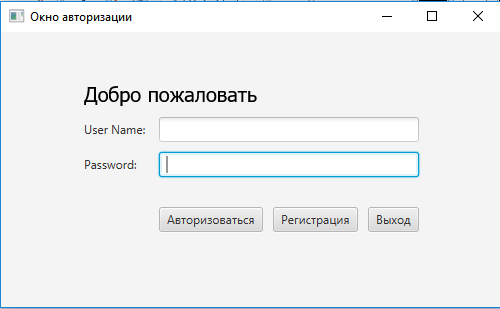
\includegraphics[scale=0.5]{img/login_form.png}
   		\caption{Окно авторизации}
   		\label{fig:login_form}
    \end{figure}
\end{center}
\begin{center}
	\begin{figure}[h!]
		\centering
   		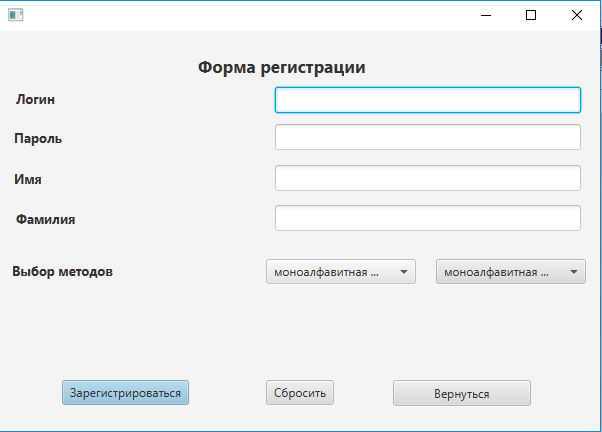
\includegraphics[scale=0.5]{img/registry_form.png}
   		\caption{Окно регистрации}
   		\label{fig:registry_form}
    \end{figure}
\end{center}
\par После прохождения авторизации пользователю открывается главное окно приложения, в котором ему, из списка методов шифрования, будут доступны лишь те методы, которые были выбраны им на этапе регистрации (рис. \ref{fig:main_form}).
\begin{center}
	\begin{figure}[h!]
		\centering
   		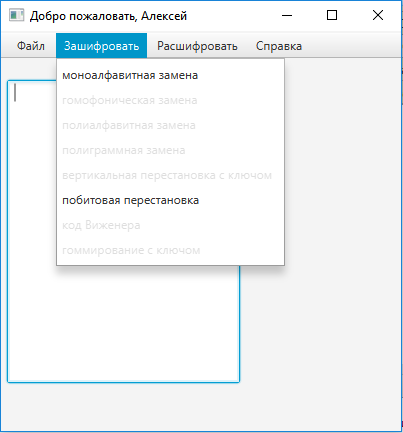
\includegraphics[scale=0.5]{img/main_form.png}
   		\caption{Главное окно программы}
   		\label{fig:main_form}
    \end{figure}
\end{center}

\begin{center}
	\begin{figure}[h!]
		\centering
   		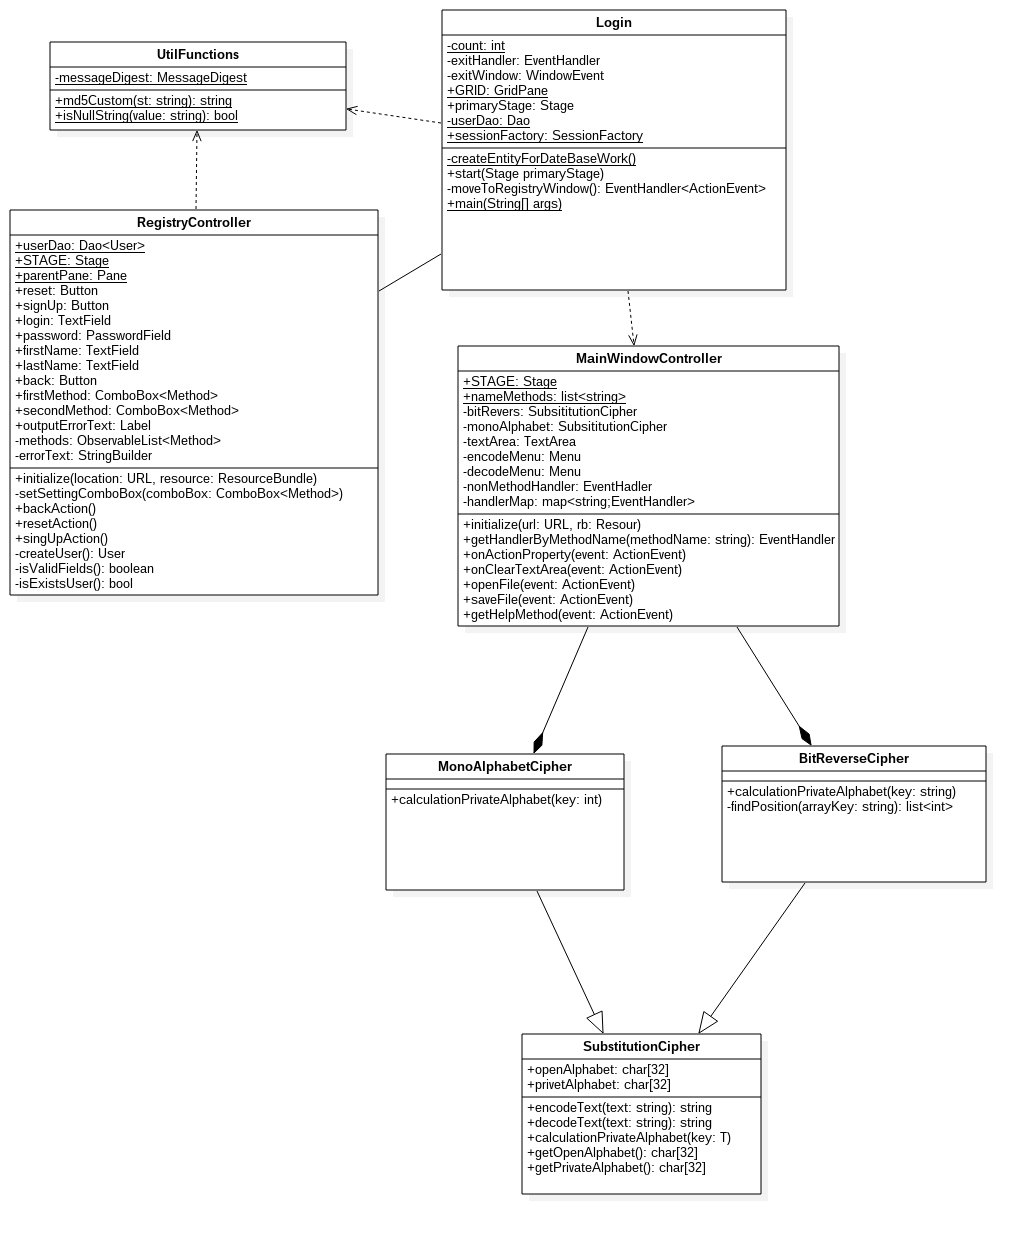
\includegraphics[scale=0.5]{img/class_diagram.png}
   		\caption{Диаграмма классов проекта}
   		\label{fig:class_diagram}
    \end{figure}
\end{center}

\subsection{Ограничения для шифруемого/расшифруемого текста}
Текст принимаемый методами шифрования состоит из строчных букв русского алфавита, из которого изключены буквы 'ё' и 'й', а так же пробел. Оставшиеся символы не входят в состав открытого алфавита, поэтому при их использовании в тексте пользователь увидит следующее сообщение: "Недопустимый символ. Расшифровка/Шифрование не возможно" (Последнее предложение зависит от выбранного пользователем метода). Пример на рис. \ref{fig:wrong_char_and_response}.
\begin{center}
	\begin{figure}[h!]
		\centering
		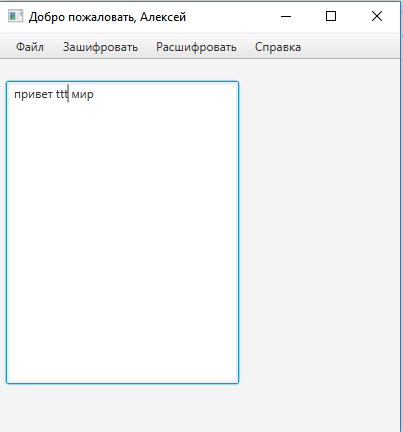
\includegraphics[scale=0.7]{img/wrong_char.png}
		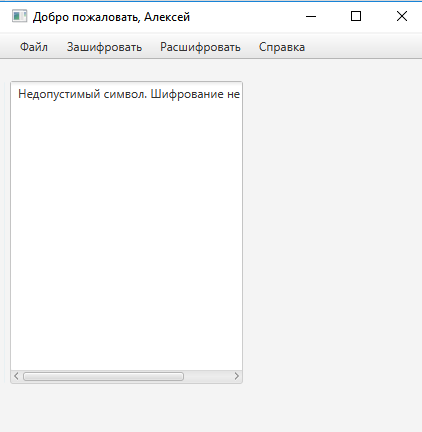
\includegraphics[scale=0.7]{img/wrong_char_response.png}
		\caption{Не верный символ в тексте}
		\label{fig:wrong_char_and_response}
	\end{figure}
\end{center}

\subsection{Системные требования}
Требования к используемому ПК:
\begin{enumerate}
\item ЦП не ниже Pentium 2 266 МГц.
\item Не менее 512 МБ ОЗУ.
\item Разрешение экрана не мение 800x600.
\item OC Windows 7, 8.x, 10; либо Mac OS X 10.8.3 или новее; либо Ubuntu 14.x или новее.
\item Java 8.
\end{enumerate}


\newpage\section{Общее описание тестирования}
Тестирование программного обеспечения – это процесс исследования и испытания программного продукта, имеющий две различные цели: 
\begin{itemize}
\item[•]Демонстрация разработчикам и заказчикам того, что программа соответствует требованиям;
\item[•]Выявлений ситуаций, в которых поведение программы является неправильным, нежелательным или несоответствующим спецификации.
\end{itemize}
Существует большое количество классификаций видов тестирования. В данной работе мы будем использовать классифакацию по степени изолированности компонентов, которая включает в себя: 
\begin{enumerate}
\item Модульное тестирование - процесс в программировании, позволяющий проверить на корректность отдельные модули исходного кода программы.
\item Интеграционное тестирование - то тестирование программного обеспечения, выполняемое на полной, интегрированной системе, с целью проверки соответствия системы исходным требованиям.
\item Системное тестирование - одна из фаз тестирования программного обеспечения, при которой отдельные программные модули объединяются и тестируются в группе.
\end{enumerate}
\par При тестировании программного проекта в данной курсовой работе, тесты писались позже, чем был реализован весь функционал приложения. Но в следствии написания тестов, многие классы были изменены и перепроектированы для более удобного проведения тестирования.
Для разработки системы тестирования были использованы следующие библиотеки:
\begin{enumerate}
\item TestFX - для автоматизированой проверки графического интерфейса (GUI), с которым взаимодействует пользователь.
\item JUnit - для проверки взаимодействия классов друг с другом, а так же для проверки отдельно взятых частей программы.
\end{enumerate}
\par При тестировании было применено ручное тестирование, для проверки зиписи текста в файл, а так же его чтения из файла. Ручное тестирование так же применялось для тестирования интерфейса. 
\par Для проверки содержимого БД использовался просмотрщик БД ИСР IntellijIdea.

\newpage \section{Модульное тестирование}
\subsection{Общее описание}
Целью модульного тестирования является проверка корректности работы отдельных функций классов программы.
Для его проведения использована библиотека jUnit, а также TestFX для моделирования работы пользователя с интерфейсом программы (GUI). При интеграционном и системном тестировании были использованы те же библиотеки, но при этом моделировалось взаимодействие классов программы как друг с другом, так и с СУБД. Поэтому для проведения этих этапов тестирования был разработан один набор классов для тестирования GUI, набор данных классов представлен на рис. \ref{fig:class_diagram_tests_gui}. Атрибуты и методы классов упущены на данной диаграмме.

\begin{center}
	\begin{figure}[h!]
		\centering
		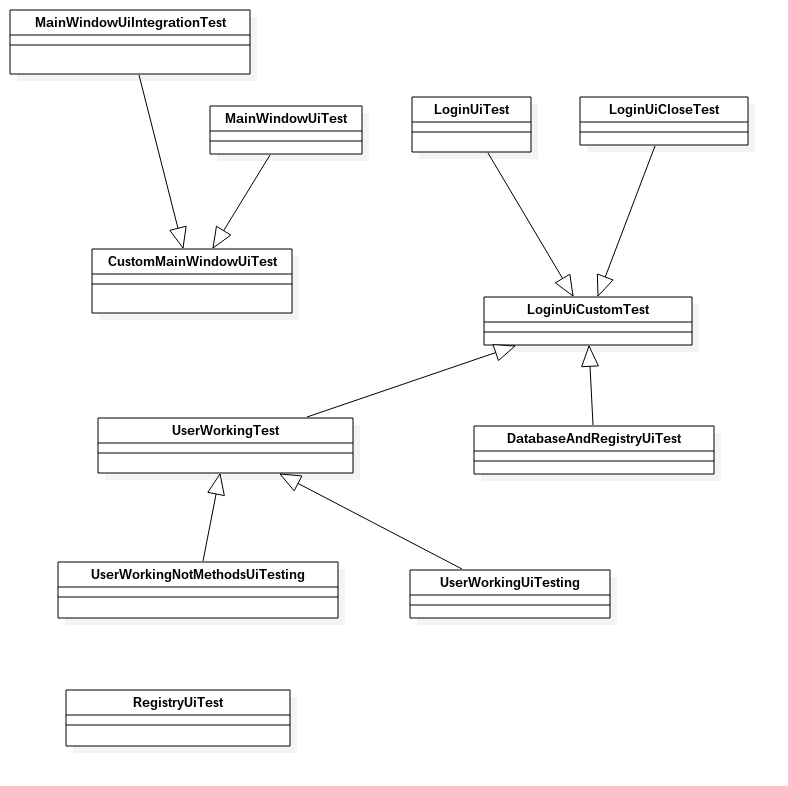
\includegraphics[scale=0.6]{img/class_diagram_ui_tests.png}
		\caption{Диаграмма классов для тестирования GUI}
		\label{fig:class_diagram_tests_gui}
	\end{figure}
\end{center}

Для модульного тестирования классов шифрования, базы данных, дополнительных функций для работы программы были разработы дополнительные классы: UtilFunctionsTest, BitReversCipherTest, MonoAlphabetCipherTest, DataBaseTesting.

\newpage\subsection{Описание методов и тестов класса MonoAlphabetCipher}
\subsubsection{Метод createOpenAlphabet}
Метод инициализирует массив допустимых символов. Сначала должен быть пробел, потом символы 'a' - 'я' заисключением символов 'ё' и 'й'. Исходный код представлен в листинге \ref{listing:createOpenAlphabet}. Метод унаследован их базового класса.
\begin{lstlisting}[language=java, caption=метод createOpenAlphabet, label = listing:createOpenAlphabet]
	private void createOpenAlphabet() {
        openAlphabet[0] = '\u0020';
        for (int i = 0; i < 9; i++) {
            openAlphabet[i + 1] = (char) ('а' + i);
        }
        for (int i = 10; i < 32; ++i) {
            openAlphabet[i] = (char) ('а' + i);
        }
    }
\end{lstlisting}
Необходимо проверить привильность инициализации, это сделано в листинге \ref{listing:testCalculationPrivateAlphabet}
\subsection{Метод calculationPrivateAlphabet}
Вычисляет закрытый алфавит на основании ключа шифрования (целое число, не превышающее мо модулю $10^9$) (листинг \ref{listing:calculationPrivateAlphabet}). Затем при шифровании символ, имеющий позицию i в OpenAlphabet заменяется символом с этим же номером из массива PrivetAlphabet.
\begin{lstlisting}[language=java, caption=метод calculationPrivateAlphabet, label = listing:calculationPrivateAlphabet]
	@Override
    public void calculationPrivateAlphabet(Integer key) {
        for (int i = 0; i < 32; i++) {
            privateAlphabet[i] = openAlphabet[Math.floorMod(i + key, 32)];
        }
    }
    
\end{lstlisting}
Необходимо проверитть правильность генерации закрытого и открытого алфавита. это делает следующий метод (листинг \ref{listing:testCalculationPrivateAlphabet}). Закрый алфавит созданый по ключу 0 должен совпадать с открытым ключом.
\begin{lstlisting}[language=java, caption=метод теста testCalculationPrivateAlphabet, label = listing:testCalculationPrivateAlphabet]
@Test
    public void testCalculationPrivateAlphabet() {
        char[] actuals = {' ', 'а', 'б', 'в', 'г', 'д', 'е', 'ж', 'з', 'и', 'к', 'л', 'м', 'н', 'о', 'п', 'р', 'с', 'т', 'у', 'ф', 'х', 'ц', 'ч', 'ш', 'щ', 'ъ', 'ы', 'ь', 'э', 'ю', 'я'};
        monoAlphabetCipher.calculationPrivateAlphabet(0);
        assertArrayEquals(monoAlphabetCipher.getPrivateAlphabet(), actuals);
        assertArrayEquals(monoAlphabetCipher.getOpenAlphabet(), actuals);
        assertArrayEquals(monoAlphabetCipher.getOpenAlphabet(), monoAlphabetCipher.getOpenAlphabet());
    }
\end{lstlisting}
Далее проверка генерации закрытого алфавита при ненулевом ключе (листинг \ref{listing:testCalculationPrivateAlphabetCaesarCipher}).
\begin{lstlisting}[language=java, caption=метод теста testCalculationPrivateAlphabet, label = listing:testCalculationPrivateAlphabetCaesarCipher]
	@Test
    public void testCalculationPrivateAlphabetCaesarCipher() {
        char[] actuals = {'в', 'г', 'д', 'е', 'ж', 'з', 'и', 'к', 'л', 'м', 'н', 'о', 'п', 'р', 'с', 'т', 'у', 'ф', 'х', 'ц', 'ч', 'ш', 'щ', 'ъ', 'ы', 'ь', 'э', 'ю', 'я', ' ', 'а', 'б'};
        monoAlphabetCipher.calculationPrivateAlphabet(3);
        assertArrayEquals(monoAlphabetCipher.getPrivateAlphabet(), actuals);
\end{lstlisting}
Тестируем возвращает ли метод исключение при некорректном значении ключа (листинг \ref{listing1:testExceptions}).
\begin{lstlisting}[language=java, caption=методы проверки исключений, label = listing1:testExceptions]
	@Test(expected = NullPointerException.class)
    public void testNullCalculationPrivateAlphabet() {
        monoAlphabetCipher.calculationPrivateAlphabet(null);
    }

    @Test(expected = ClassCastException.class)
    public void testWrongArgumentCalculationPrivateAlphabet() {
        monoAlphabetCipher.calculationPrivateAlphabet("test");
    }
\end{lstlisting}
\subsubsection{Метод encodeText и decodeText}
Выполняют шифрование и дешифрование текста. Эти методы унаследованы из базового класса (листинг \ref{listing1:encodeAndDecode}). Если переданная строка содержит символы, недопустимые в данном алфавите, то метод должен вернуть строку "Недопустимый символ. Шифрование/Дешифрование не возможно".
\begin{lstlisting}[language=java, caption=методы encode и decode, label = listing1:encodeAndDecode]
     /**
     * Закодировать текст
     *
     * @param originalText текст
     * @return закодированный текст
     */
    public String encodeText(String originalText) {
        originalText = originalText.replaceAll("\n", " ").toLowerCase();
        char[] text = originalText.toCharArray();
        char[] result = new char[text.length];
        int index;
        for (int i = 0; i < text.length; i++) {
            index = contains(openAlphabet, text[i]);
            if (index < 0) return "Недопустимый символ. Шифрование не возможно";
            result[i] = privateAlphabet[index];
        }
        return String.valueOf(result);
    }

    /**
     * Раскодировать текст
     *
     * @param originalText текст
     * @return раскодированный текст
     */
    public String decodeText(String originalText) {
        char[] text = originalText.toCharArray();
        char[] result = new char[text.length];
        int index;
        for (int i = 0; i < text.length; i++) {
            index = contains(privateAlphabet, text[i]);
            if (index < 0) return "Недопустимый символ. Расшифровка не возможно";
            result[i] = openAlphabet[index];
        }
        return String.valueOf(result);
    }

    private int contains(char[] chars, char symbol) {
        for (int i = 0; i < chars.length; i++) {
            if (chars[i] == symbol) {
                return i;
            }
        }
        return -1;
    }
\end{lstlisting}
Необходимо проверить корректность шифрования. Это делают следующие методы (листинг \ref{listing1:testEncocodeAndDecode}).
\begin{lstlisting}[language=java, caption=методы проверки корректности шифрования/дешифрования, label = listing1:testEncocodeAndDecode]
    @Test
    public void testEncodeText() {
        monoAlphabetCipher.calculationPrivateAlphabet(3);
        assertEquals(monoAlphabetCipher.encodeText("тест"), "хифх");
    }

    @Test
    public void testEncodeAndDecode() {
        monoAlphabetCipher.calculationPrivateAlphabet(30);
        String encode = monoAlphabetCipher.encodeText("тест");
        assertEquals("тест", monoAlphabetCipher.decodeText(encode));
    }

\end{lstlisting}
А также корректность певедения метода при недопустимой строке (листинг \ref{listing1:testWrongCharInEncodeAndDecodeText}).
\begin{lstlisting}[language=java, caption=методы проверки корректности шифрования/дешифрования, label = listing1:testWrongCharInEncodeAndDecodeText]
    @Test
    public void testWrongCharInEncodeAndDecodeText() {
        monoAlphabetCipher.calculationPrivateAlphabet(1);
        Assert.assertEquals(monoAlphabetCipher.encodeText("tttt"), "Недопустимый символ. Шифрование не возможно");
        Assert.assertEquals(monoAlphabetCipher.encodeText("й"), "Недопустимый символ. Шифрование не возможно");
        Assert.assertEquals(monoAlphabetCipher.encodeText("ё"), "Недопустимый символ. Шифрование не возможно");
        Assert.assertEquals(monoAlphabetCipher.encodeText("-"), "Недопустимый символ. Шифрование не возможно");
        Assert.assertEquals(monoAlphabetCipher.encodeText("+"), "Недопустимый символ. Шифрование не возможно");
        Assert.assertEquals(monoAlphabetCipher.decodeText("tttt"), "Недопустимый символ. Расшифровка не возможно");
        Assert.assertEquals(monoAlphabetCipher.decodeText("й"), "Недопустимый символ. Расшифровка не возможно");
        Assert.assertEquals(monoAlphabetCipher.decodeText("ё"), "Недопустимый символ. Расшифровка не возможно");
        Assert.assertEquals(monoAlphabetCipher.decodeText("-"), "Недопустимый символ. Расшифровка не возможно");
        Assert.assertEquals(monoAlphabetCipher.decodeText("+"), "Недопустимый символ. Расшифровка не возможно");
    }
\end{lstlisting}
\newpage\subsection{Описание методов и тестов класса BitReverseCipher}
Данный класс выполняет шифрование/дешифрование методом побитовой перестановки. Ключём шифрования является строка являющаяся перестановкий "12345", которая задаёт правило перестановки битов для каждого символа. Напимер строка "54312" означает, что 5-й бит будет переставлен на 1 место (нумерация от 1 до 5), 4-й бит на 2-e место, 3-й бит остаётся на месте, 1-й бит идёт на 4 место, 2-й бит на 5-е.
\par Далее описаны методы, которые переопределены у базового класса.
\subsubsection{Метод findPosition}
Метод на основе ключа генерирует массив, с правилами переставки битов в исходных символов (листинг \ref{listing2:findPosition}).
\begin{lstlisting}[language=java, caption=метод findPosition, label=listing2:findPosition]
    private int[] findPosition(String arrayKey) {
        int[] result = new int[arrayKey.length()];
        result[0] = arrayKey.indexOf("1");
        result[1] = arrayKey.indexOf("2");
        result[2] = arrayKey.indexOf("3");
        result[3] = arrayKey.indexOf("4");
        result[4] = arrayKey.indexOf("5");
        return result;
    }
\end{lstlisting}
Корректнгость данного метода проверяется при описанного дальше метода.
\subsubsection{Метод calculationPrivateAlphabet}
Метод генерирует закрытый алфавит. На вход подаётся строка с ключём (листинг \ref{listing2:calculationPrivateAlphabet}).
\begin{lstlisting}[language=java, caption=метод calculationPrivateAlphabet, label=listing2:calculationPrivateAlphabet]
    public void calculationPrivateAlphabet (String key) {
        int[] arrayKey = findPosition(key);
        for (int i = 0; i < 32; i++) {
            StringBuilder stI = new StringBuilder(Integer.toBinaryString(i));
            for (int j = stI.length(); j < 5; j++) {
                stI.insert(0, "0");
            }
            StringBuilder charAlph = new StringBuilder();
            char[] mass = stI.toString().toCharArray();
            for (int anArrayKey : arrayKey) {
                charAlph.append(mass[anArrayKey]);
            }
            int exitI = Integer.parseInt(charAlph.toString(), 2);
            privateAlphabet[i] = openAlphabet[exitI];
        }
    }
\end{lstlisting}

Можно заметить, что шифрование пробела всегда приведёт к пробельному символу(код 0). Для проверки этого разработаен следующий метод (листинг \ref{listing2:testFirstElementPrivateAlphabetAtAnyKey}).
\begin{lstlisting}[language=java, caption=метод calculationPrivateAlphabet, label=listing2:testFirstElementPrivateAlphabetAtAnyKey]
    @Test
    public void testFirstElementPrivateAlphabetAtAnyKey() {
        bitReversCipher.calculationPrivateAlphabet("54321");
        assertEquals(bitReversCipher.getPrivateAlphabet()[0], ' ');
        bitReversCipher.calculationPrivateAlphabet("53241");
        assertEquals(bitReversCipher.getPrivateAlphabet()[0], ' ');
        bitReversCipher.calculationPrivateAlphabet("13425");
        assertEquals(bitReversCipher.getPrivateAlphabet()[0], ' ');
        bitReversCipher.calculationPrivateAlphabet("31245");
        assertEquals(bitReversCipher.getPrivateAlphabet()[0], ' ');
    }
\end{lstlisting}

Далее проверить в целом построение закрытого и открытого алфавита (листинг \ref{listing2:testCalculationPrivateAlphabet}).
\begin{lstlisting}[language=java, caption=метод calculationPrivateAlphabet, label=listing2:testCalculationPrivateAlphabet]
    @Test
    public void testCalculationPrivateAlphabetEqualsOpenAlphabet() {
        char[] actuals = {' ', 'а', 'б', 'в', 'г', 'д', 'е', 'ж', 'з', 'и', 'к', 'л', 'м', 'н', 'о', 'п', 'р', 'с', 'т', 'у', 'ф', 'х', 'ц', 'ч', 'ш', 'щ', 'ъ', 'ы', 'ь', 'э', 'ю', 'я'};
        bitReversCipher.calculationPrivateAlphabet("12345");
        assertArrayEquals(bitReversCipher.getPrivateAlphabet(), actuals);
        assertArrayEquals(bitReversCipher.getOpenAlphabet(), actuals);
        assertArrayEquals(bitReversCipher.getOpenAlphabet(), bitReversCipher.getOpenAlphabet());
    }

    @Test
    public void testCalculationPrivateAlphabet() {
        char[] actuals = {' ', 'р', 'з', 'ш', 'г', 'ф', 'м', 'ь', 'б', 'т', 'к', 'ъ', 'е', 'ц', 'о', 'ю', 'а', 'с', 'и', 'щ', 'д', 'х', 'н', 'э', 'в', 'у', 'л', 'ы', 'ж', 'ч', 'п', 'я'};
        bitReversCipher.calculationPrivateAlphabet("54321");
        assertArrayEquals(bitReversCipher.getPrivateAlphabet(), actuals);
    }
\end{lstlisting}
Затем можно проверить, что при некорректном значии ключа происходят исключения (листинг \ref{listing2:testWrongValueForCalculationPrivateAlphabet}).
\begin{lstlisting}[language=java, caption=метод calculationPrivateAlphabet, label=listing2:testWrongValueForCalculationPrivateAlphabet]
    @Test(expected = IndexOutOfBoundsException.class)
    public void testWrongValueForCalculationPrivateAlphabet() {
        bitReversCipher.calculationPrivateAlphabet("00000");
    }

    @Test(expected = ClassCastException.class)
    public void testWrongArgumentForCalculationPrivateAlphabet() {
        bitReversCipher.calculationPrivateAlphabet(1213234);
    }
\end{lstlisting}

\subsubsection{Тестирование остальных методов}

Далее необходимо проверить правальность шифрования и расшифрования строки (листинг \ref{listing2:testEncodeDecode}).
\begin{lstlisting}[language=java, caption=метод calculationPrivateAlphabet, label=listing2:testEncodeDecode]
	@Test
    public void testEncode() {
        bitReversCipher.calculationPrivateAlphabet("54321");
        assertEquals(bitReversCipher.encodeText("тест"), "имси");
    }

    @Test
    public void testEncodeDecode() {
        bitReversCipher.calculationPrivateAlphabet("54321");
        String encode = bitReversCipher.encodeText("тест");
        assertEquals(bitReversCipher.decodeText(encode), "тест");
    }
\end{lstlisting}
Проверка поведения при некоректном шифруемом/дешифруемом тексте (листинг \ref{listing2:testWrongCharInEncodeAndDecodeText}).
\begin{lstlisting}[language=java, caption=метод calculationPrivateAlphabet, label=listing2:testWrongCharInEncodeAndDecodeText]
    @Test
    public void testWrongCharInEncodeAndDecodeText() {
        bitReversCipher.calculationPrivateAlphabet("54321");
        Assert.assertEquals(bitReversCipher.encodeText("tttt"), "Недопустимый символ. Шифрование не возможно");
        Assert.assertEquals(bitReversCipher.encodeText("й"), "Недопустимый символ. Шифрование не возможно");
        Assert.assertEquals(bitReversCipher.encodeText("ё"), "Недопустимый символ. Шифрование не возможно");
        Assert.assertEquals(bitReversCipher.encodeText("-"), "Недопустимый символ. Шифрование не возможно");
        Assert.assertEquals(bitReversCipher.encodeText("+"), "Недопустимый символ. Шифрование не возможно");
        Assert.assertEquals(bitReversCipher.decodeText("tttt"), "Недопустимый символ. Расшифровка не возможно");
        Assert.assertEquals(bitReversCipher.decodeText("й"), "Недопустимый символ. Расшифровка не возможно");
        Assert.assertEquals(bitReversCipher.decodeText("ё"), "Недопустимый символ. Расшифровка не возможно");
        Assert.assertEquals(bitReversCipher.decodeText("-"), "Недопустимый символ. Расшифровка не возможно");
        Assert.assertEquals(bitReversCipher.decodeText("+"), "Недопустимый символ. Расшифровка не возможно");
    }
\end{lstlisting}

\subsection{Описание методов и тестов класса UtilFunctions}

Данный класс реализует функции, необходимые во многих модулях проекта. А именно проверку строки на пустоту и MD5 хеширование(применяется для хранения паролей). Необходимо проверить эту функциональнсть, для чего и разработан класс UtilFunctionsTest.
\par Тестирование md5 представлено в листинге \ref{listing:testMd5}.

\begin{lstlisting}[language=java, caption=тестирование md5 , label=listing:testMd5]
    @Test
    public void md5EqualsTesting() {
        String expected = md5Custom("1");
        assertEquals(expected, "c4ca4238a0b923820dcc509a6f75849b");
        expected = md5Custom("md5test");
        assertEquals(expected, "82da61aa724b5d149a9c5dc8682c2a45");
        expected = md5Custom("абра-кадбра, магия какая-то");
        assertEquals(expected, "783e47ca544ddf34ccce81b524adbbe3");
    }

    @Test
    public void md5NullArgument() {
        assertEquals(md5Custom(null), "");
    }

\end{lstlisting}


Тестирование метода проверки строки на пустоту представлено в листинге \ref{listing:testIsNullString}

\begin{lstlisting}[language=java, caption=тестирование isNullString, label=listing:testIsNullString]
    @Test
    public void isNullStringTest() {
        assertEquals(isNullString(null), true);
        assertEquals(isNullString(""), true);
        assertEquals(isNullString("          "), true);
        assertEquals(isNullString("    dsfsdf   "), false);
        assertEquals(isNullString("тестовое значение"), false);
        assertEquals(isNullString(" "), true);
    }
\end{lstlisting}

\subsection{Описание тестирования класса RegistryController}
Данный класс отвечает за окно регистрации пользователя и за взаимодействие с БД во время регистрации.
Тестирование осуществлялось с помощью моделирования рботы пользователя с GUI (TestFX). Для регистрации необходимо как минимум заполнить поля "Логин" и "Пароль", поэтому необходимо протестировать, что при попытке регистрации не указав хотя бы одно из этих полей будет выведено соответствующее сообщение. Это тестирование выполняет класс RegistryUiTest (листинг \ref{listing:testNullFields}). Также необходимо протестировать поведение программы при попытке зарегистрировать пользователя, логин которого совпадает с зарегестрированным ранее. Это выполняет класс DatabaseAndRegistryUiTest (листинг \ref{listing:testRegExistUser}).

\begin{lstlisting}[language=java, caption=тестирование не заполнения полей при регистрации, label=listing:testNullFields]
public class RegistryUiTest extends GuiTest {
    private static FxRobot robot;
    private Label outputErrorText;

    @BeforeClass
    public static void createRobot() {
        robot = new FxRobot();
    }

    @Before
    public void getOutputErrorText() {
        outputErrorText =  find("#outputErrorText");
    }

    @After
    public void clickResetField() {
        robot.clickOn("#reset");
    }

    @Override
    protected Parent getRootNode() {
        Parent parent = null;
        try {
            parent = FXMLLoader.load(getClass().getResource("/fxml/Registry.fxml"));
            return parent;
        } catch (IOException ex) {
            // TODO ...
        }
        return parent;
    }


    @Test
    public void emptyLoginAndPasswordFieldTest() {
        robot.clickOn("#signUp").sleep(500);
        Assert.assertEquals(outputErrorText.getText(), "Не заполнены обязательные поля: Логин; Пароль; ");
    }

    @Test
    public void emptyLoginFieldTest() {
        robot.clickOn("#login").write("notEmptyLogin");
        robot.clickOn("#signUp");
        Assert.assertEquals(outputErrorText.getText(), "Не заполнены обязательные поля: Пароль; ");
    }

    @Test
    public void emptyPasswordFieldTest() {
        robot.clickOn("#password").write("tesPass");
        robot.clickOn("#signUp");
        Assert.assertEquals(outputErrorText.getText(), "Не заполнены обязательные поля: Логин; ");
    }
}

\end{lstlisting}

\begin{lstlisting}[language=java, caption=тестирование попытки регистрации существующего пользователя, label=listing:testRegExistUser]
public class DatabaseAndRegistryUiTest extends LoginUiCustomTest {

    @Test
    public void userExistsTest() {
        clickOn(registry);
        clickOn("#login").write("Aleksey");
        clickOn("#password").write("tesPass");
        clickOn("#signUp");
        Label outputErrorText = find("#outputErrorText");
        Assert.assertEquals(outputErrorText.getText(), "Пользователь с логином: Aleksey существует!");
        closeRegistryWindowAndTest();
    }


}

\end{lstlisting}

\subsection{Описание тестирования класса MainWindowController}
Данный класс отвечает за главное окно программы. Необходимо проверить, корректность его работы. Это сделано в классе MainWindowUiTest, который описан в листинге \ref{listing:testMainWindow}. А именно проверить корректность работы поля memo, работу кнопки "Очистить", и что по умолчанию не доступен ни один метод шифрования и дешифрования.

\begin{lstlisting}[language=java, caption=тестирование MainWindow, label=listing:testMainWindow]
public class MainWindowUiTest extends CustomMainWindowUiTest {
    private TextArea textArea;

    @Before
    public void findTextArea() {
        textArea = find("#textArea");
    }

    @Override
    protected Parent getRootNode() {
        Parent parent = null;
        try {
            parent = FXMLLoader.load(getClass().getResource("/fxml/MainWindow.fxml"));
            return parent;
        } catch (IOException ex) {
            // TODO ...
        }
        return parent;
    }

    @Test
    public void writeInTextAreaTest() {
        robot.clickOn(textArea).write("авыаыва");
        verifyThat(textArea, hasText("авыаыва"));
    }

    @Test
    public void clickAllEncodeMenuTest() {
        robot.clickOn("#encodeMenu");
        clickAllMethodsMenu("encode");
        robot.clickOn("#encodeMenu");
    }

    @Test
    public void clickAllDecodeMenuTest() {
        robot.clickOn("#decodeMenu");
        clickAllMethodsMenu("decode");
        robot.clickOn("#decodeMenu");
    }

    private static void clickAllMethodsMenu(String variantName) {
        String itemId;
        for (String name : methodNames) {
            itemId = "#" + variantName + name;
            robot.clickOn(itemId);
        }
    }
    @Test
    public void clearTextArea() {
        String testText = "текстовый текст, для проверки очистки области ввода текста";
        robot.clickOn(textArea).write(testText);
        verifyThat(textArea, hasText(testText));
        robot.clickOn("#fileMenu").clickOn("#clear");
        verifyThat(textArea, hasText(""));
    }
}
\end{lstlisting}

\newpage\subsection{Результаты тестирования и выводы на данном этапе}
Результаты прохождения тестов представлены в таблицах \ref{table:unit_testing_MonoAlphabetCipherTest} - \ref{table:unit_testing_UtilFunctionsTest}.

Все тесты были пройдены успешно, ошибок не было обнаружено.

\begin{table}[h]
	\caption{Прохождение тестов класса MonoAlphabetCipherTest}
	\centering
	\begin{tabular}{|c|l|l|}
	\hline 
	№ &  Название теста & Результат \\ 
	\hline 
	1 &  testNullCalculationPrivateAlphabet & Успешно пройден  \\
	\hline 
	2 &  testWrongArgumentCalculationPrivateAlphabet & Успешно пройден  \\
	\hline 
	3 & testCalculationPrivateAlphabet & Успешно пройден  \\
	\hline 
	4 & testCalculationPrivateAlphabetCaesarCipher & Успешно пройден  \\
	\hline 
	5 & testEncodeText & Успешно пройден  \\
	\hline 
	6 & testEncodeAndDecode & Успешно пройден  \\
	\hline 
	7 & testWrongCharInEncodeAndDecodeText & Успешно пройден  \\
	\hline 
\end{tabular} 
\label{table:unit_testing_MonoAlphabetCipherTest} 
\end{table}

\begin{table}[h]
	\caption{Прохождение тестов класса BitReversCipherTest}
	\centering
	\begin{tabular}{|c|l|l|}
	\hline 
	№ &  Название теста & Результат \\ 
	\hline 
	8 &  testCalculationPrivateAlphabetEqualsOpenAlphabet & Успешно пройден  \\
	\hline 
	9 &  testCalculationPrivateAlphabet & Успешно пройден  \\
	\hline 
	10 & testFirstElementPrivateAlphabetAtAnyKey & Успешно пройден  \\
	\hline 
	11 & testLastElementPrivateAlphabetAtAnyKey & Успешно пройден  \\
	\hline 
	12 & testEncode & Успешно пройден  \\
	\hline 
	13 & testEncodeDecode & Успешно пройден  \\
	\hline 
	14 & testWrongValueForCalculationPrivateAlphabet & Успешно пройден  \\
	\hline 
	15 & testWrongArgumentForCalculationPrivateAlphabet & Успешно пройден  \\
	\hline 
	16 & testWrongCharInEncodeAndDecodeText & Успешно пройден  \\
	\hline 
\end{tabular} 
\label{table:unit_testing_BitReversCipherTest} 
\end{table}

\begin{table}[h]
	\caption{Прохождение тестов класса UtilFunctionsTest}
	\centering
	\begin{tabular}{|c|l|l|}
	\hline 
	№ &  Название теста & Результат \\ 
	\hline 
	17 &  md5EqualsTesting & Успешно пройден  \\
	\hline 
	18 &  md5NullArgument & Успешно пройден  \\
	\hline 
	19 & isNullStringTest & Успешно пройден  \\
	\hline 
\end{tabular} 
\label{table:unit_testing_UtilFunctionsTest} 
\end{table}

\begin{table}[pt!]
	\caption{Прохождение GUI тестов при модульном тестировании}
	\centering
	\begin{tabular}{|c|l|l|}
	\hline 
	№ &  Название теста & Результат \\ 
	\hline 
	\multicolumn{3}{|c|}{Класс \textbf{RegistryUiTest}}\\
	\hline
	17 &  emptyLoginAndPasswordFieldTest & Успешно пройден  \\
	\hline 
	18 &  emptyLoginFieldTest & Успешно пройден  \\
	\hline 
	19 & emptyPasswordFieldTest & Успешно пройден  \\
	\hline 
	\multicolumn{3}{|c|}{Класс \textbf{DatabaseAndRegistryUiTest}}\\
	\hline
	20 & userExistsTest & Успешно пройден  \\
	\hline 
	\multicolumn{3}{|c|}{Класс \textbf{MainWindowUiTest}}\\
	\hline
	21 & writeInTextAreaTest & Успешно пройден  \\
	\hline
	22 & clickAllEncodeMenuTest & Успешно пройден  \\
	\hline
	23 & clickAllDecodeMenuTest & Успешно пройден  \\
	\hline
	24 & clearTextArea & Успешно пройден  \\
	\hline
\end{tabular} 
\label{table:unit_testing_UtilFunctionsTest} 
\end{table}

\newpage \section{Интеграционное тестирование}
\subsection{Общее описание}
Целью интеграционного тестирования является проверка всех возможных непосредвенных взаимодействий классов программы друг с другом. 
Для его проведения использованы следующие библиотеки: JUnit и TestFX.
Были разработаны класс IntegrationCipherTest, а также представленные на рис. \ref{fig:class_diagram_tests_gui} классы MainWindowUiIntegrationTest, LoginUiTest, LoginUiCloseTest, UserWorkingNotMethodsUiTesting, UserWorkingUiTesting.

\newpage\subsection{Тестирование взаимодействия класса Login}
Login - это главный класс приложения, который запускает его и одновременно является контроллером для окна авторизации. Пользователь должен пройти авторизацию или зарегистрироваться. Если после третьей попытки не удалось авторизиваться, то программа закрывается.
\subsubsection{Закрытие программы при неверной авторизации}
С помощью TestFx моделируется попытка неудачной авторизации: три раза вводим не верный пароль. На каждом шаге проверяем появилось ли в специальной строке сообщение об ошибке: "Не верный пароль''", выделенное красным цветом. (листинг \ref{listing_login:test_wrong_authorization}).
\begin{lstlisting}[language=java, caption=Тестирование неверной авторизации, label=listing_login:test_wrong_authorization]
public class LoginUiCloseTest extends LoginUiCustomTest {
    @Test
    public void threeWrongAuthorizationTest() {
        for (int i = 0; i < 3; i++) {
            clickOn(userName).write("Aleksey");
            clickOn(password).write("tttt");
            clickOn(authorization).sleep(100);
            verifyThat(resultAuthorization, hasText("Не верный пароль"));
            assertEquals(resultAuthorization.getFill(), Color.FIREBRICK);
            userName.clear();
            password.clear();
        }
        assertEquals(stage.isShowing(), false);
        assertEquals(sessionFactory.isClosed(), true);
    }
}
\end{lstlisting}

\subsubsection{Реакция программы при неверном пароле}
При вводе корректного (существующего) логина пользователя, но некорректного пароля для него в специальной строке формы авторизации должна появиться надпись "Неверный пароль''", выделенная красным цветом. Этот (листинг \ref{listing_login:test_wrong_password}) и последующие тесты класса Login описаны в классе LoginUiTest.

\begin{lstlisting}[language=java, caption=Тестирование ввода неверного пароля, label=listing_login:test_wrong_password]      
    @Test
    public void wrongAuthorizationTest() {
        assertEquals(sessionFactory.isClosed(), false);
        clickOn(userName).write("Aleksey");
        clickOn(password).write("retdfgdfh");
        clickOn(authorization);
        verifyThat(resultAuthorization, hasText("Не верный пароль"));
        assertEquals(resultAuthorization.getFill(), Color.FIREBRICK);
    }
\end{lstlisting}

\subsubsection{Реакция программы при не существующем логине}
После нажатия на кнопку авторизации в БД ищется пользователь с указаным логином, если не возвращается пользователь с таким логином, то должно появиться сообщение: "Такого пользователя не существует" (листинг \ref{listing_login:test_wrong_user}).
\begin{lstlisting}[language=java, caption=Тестирование при несуществующем логине, label=listing_login:test_wrong_user]
    @Test
    public void thisUserDoesntExistTest() {
        assertEquals(sessionFactory.isClosed(), false);
        clickOn(userName).write("ТестНик");
        clickOn(password).write("tttt");
        clickOn(authorization);
        verifyThat(resultAuthorization, hasText("Такого пользователя не существует"));
        assertEquals(resultAuthorization.getFill(), Color.FIREBRICK);
    }
\end{lstlisting}


\subsubsection{Реакция программы при верной авторизации}
При прохождении авторизации окно авторизации должно закрыться, а вместо него должно появиться основное окно программы (листинг \ref{listing_login:test_true_autorization}). 

\begin{lstlisting}[language=java, caption=Тестирование прохождения авторизации, label=listing_login:test_true_autorization]
    @Test
    public void openMainWindowTest() {
        assertEquals(sessionFactory.isClosed(), false);
        clickOn(userName).write("Aleksey");
        clickOn(password).write("yui");
        clickOn(authorization);
        verifyThat(resultAuthorization, hasText("Пароль верный"));
        assertEquals(resultAuthorization.getFill(), Color.GREEN);
        waitUntil("#AnchorPane", visible());
    }
\end{lstlisting}

\subsubsection{Тестирование перехода к окну регистрации}
При нажатии на кнопку "'Регистация'' , должно появится соответствующее окно, а окно для авторизации исчезнуть (листинг \ref{listing_login:test_registration_to_registration}). 
\begin{lstlisting}[language=java, caption=Тестирование перехода к окну регистрации, label=listing_login:test_registration_to_registration]
	protected void openRegistryWindowAndTest() {
        clickOn(registry);
        assertEquals(gridPane.isDisable(), true);
        waitUntil("#registryPane", visible());
    }

    protected void closeRegistryWindowAndTest() {
        clickOn("#back");
        assertEquals(gridPane.isDisable(), false);
    }     
    @Test
    public void openRegistryWindowTest() {
        openRegistryWindowAndTest();
        closeRegistryWindowAndTest();
    }
\end{lstlisting}

\newpage\subsection{Тестирование взаимодействия классов \\MonoAlphabetCipher и BitReverseCipher}
Тестирование осуществляется посредством многократного шифрования и расшифрования текста различными методами. После последовательного шифрования и расшифрования разными методами с неизменными ключами текст должен совпасть с исходным. Если провести такой же тест, но при расшифровании изменить ключ одного из методов, то результат должен не совпасть с исходным. Далее проведём тест, при котором зашуфруем несколько раз обоими методами с разнами ключами и расшуфруем в обратном порядке с соответствующими ключами, результат должен совпасть с исходным. Все эти три теста описаны в классе IntegrationCipherTest, который представлен в листинге \ref{listing_cipher:test_cipher_methods}.

\begin{lstlisting}[language=java, caption=класс IntegrationCipherTest, label=listing_cipher:test_cipher_methods]
public class IntegrationCipherTest {
    private static SubstitutionCipher<Integer> monoAlphabet;
    private static SubstitutionCipher<String> bitRevers;
    private String actualText;

    @BeforeClass
    public static void test() {
        monoAlphabet = new MonoAlphabetCipher();
        bitRevers = new BitReversCipher();
    }

    @Before
    public void createCipherClass() {
        actualText = "специальныи текст для тестов";
    }

    @Test
    public void integrationCipherEqualsTest() {
        monoAlphabet.calculationPrivateAlphabet(4);
        bitRevers.calculationPrivateAlphabet("32451");
        String expectedText = monoAlphabet.encodeText(actualText);
        expectedText = bitRevers.decodeText(expectedText);
        expectedText = bitRevers.encodeText(expectedText);
        expectedText = monoAlphabet.decodeText(expectedText);
        Assert.assertEquals(expectedText, actualText);
    }

    @Test
    public void  integrationCipherNotEqualsTest() {
        monoAlphabet.calculationPrivateAlphabet(4);
        bitRevers.calculationPrivateAlphabet("32451");
        String testText = monoAlphabet.encodeText(actualText);
        testText = bitRevers.decodeText(testText);
        bitRevers.calculationPrivateAlphabet("52341");
        String expectedText = bitRevers.encodeText(testText);
        Assert.assertNotEquals(expectedText, testText);
    }

    @Test
    public void  integrationDeepCipherEqualsTest() {
        monoAlphabet.calculationPrivateAlphabet(2);
        String expectedText = monoAlphabet.encodeText(actualText);

        bitRevers.calculationPrivateAlphabet("53241");
        expectedText = bitRevers.encodeText(expectedText);
        Assert.assertNotEquals(expectedText, actualText);

        monoAlphabet.calculationPrivateAlphabet(3);
        expectedText = monoAlphabet.decodeText(expectedText);

        bitRevers.calculationPrivateAlphabet("24531");
        expectedText = bitRevers.decodeText(expectedText);
        Assert.assertNotEquals(expectedText, actualText);

        expectedText = bitRevers.encodeText(expectedText);
        expectedText = monoAlphabet.encodeText(expectedText);
        Assert.assertNotEquals(expectedText, actualText);

        bitRevers.calculationPrivateAlphabet("53241");
        expectedText = bitRevers.decodeText(expectedText);

        monoAlphabet.calculationPrivateAlphabet(2);
        expectedText = monoAlphabet.decodeText(expectedText);

        Assert.assertEquals(expectedText, actualText);
    }
}
\end{lstlisting}


\newpage\subsection{Тестирование взаимодействия класса MainWindow}
MainWindow - класс отвечающий за главное окно программы. Он взаимодействует с классами, реализующими методы шифрования. Проведём тестирование, аналогичное тестированию классов MonoAlphabetCipher и BitReverseCipher, но теперь классы для шифрования будут взаимодействовать не напрямую, а через MainWindow (как и происходит на самом деле), посредством моделирвания работы пользователя с gui. Оно представлено в листинге \ref{listing_mainWindow:MainWindowUiIntegrationTestn}. Предыдушее тестирование направлено на проверку корректности классов шифрования и их взаимодействия, а такущее преимущественно на корректность работы MainWindow с данными классами.

\begin{lstlisting}[language=java, caption=класс MainWindowUiIntegrationTest, label=listing_mainWindow:MainWindowUiIntegrationTestn]
public class MainWindowUiIntegrationTest extends CustomMainWindowUiTest {
    private TextArea textArea;
    String actualText;

    @BeforeClass
    public static void mainWindowSettings() {
        MainWindowController.nameMethods = Arrays.asList(
                methodNames.get(0), methodNames.get(5)
        );
    }

    @Before
    public void findTextArea() {
        textArea = find("#textArea");
        actualText = "специальныи текст для тестов";
        robot.clickOn(textArea).write(actualText);
    }

    @After
    public void clearTextArea() {
        textArea.clear();
    }

    @Test
    public void integrationCipherEqualsTest() {
        robot.clickOn("#encodeMenu").clickOn("#encodeMonoAlphabet")
                .clickOn("#txtFieldDialog").write('4').clickOn("#okDialog");
        robot.clickOn("#decodeMenu").clickOn("#decodeBitRevers")
                .clickOn("#txtFieldDialog").write("32451").clickOn("#okDialog");
        robot.clickOn("#encodeMenu").clickOn("#encodeBitRevers")
                .clickOn("#txtFieldDialog").write("32451").clickOn("#okDialog");
        robot.clickOn("#decodeMenu").clickOn("#decodeMonoAlphabet")
                .clickOn("#txtFieldDialog").write('4').clickOn("#okDialog");
        Assert.assertEquals(textArea.getText(), actualText);
    }

    @Test
    public void integrationCipherNotEqualsTest() {
        robot.clickOn("#encodeMenu").clickOn("#encodeMonoAlphabet")
                .clickOn("#txtFieldDialog").write('4').clickOn("#okDialog");
        robot.clickOn("#decodeMenu").clickOn("#decodeBitRevers")
                .clickOn("#txtFieldDialog").write("32451").clickOn("#okDialog");
        String testText = textArea.getText();
        robot.clickOn("#decodeMenu").clickOn("#decodeBitRevers")
                .clickOn("#txtFieldDialog").write("52341").clickOn("#okDialog");
        Assert.assertNotEquals(textArea.getText(), testText);
    }

    @Test
    public void  integrationDeepCipherEqualsTest() {
        robot.clickOn("#encodeMenu").clickOn("#encodeMonoAlphabet")
                .clickOn("#txtFieldDialog").write("2").clickOn("#okDialog");
        robot.clickOn("#encodeMenu").clickOn("#encodeBitRevers")
                .clickOn("#txtFieldDialog").write("53241").clickOn("#okDialog");
        Assert.assertNotEquals(textArea.getText(), actualText);
        robot.clickOn("#decodeMenu").clickOn("#decodeMonoAlphabet")
                .clickOn("#txtFieldDialog").write('3').clickOn("#okDialog");
        robot.clickOn("#decodeMenu").clickOn("#decodeBitRevers")
                .clickOn("#txtFieldDialog").write("24531").clickOn("#okDialog");
        Assert.assertNotEquals(textArea.getText(), actualText);
        robot.clickOn("#encodeMenu").clickOn("#encodeBitRevers")
                .clickOn("#txtFieldDialog").write("24531").clickOn("#okDialog");
        robot.clickOn("#encodeMenu").clickOn("#encodeMonoAlphabet")
                .clickOn("#txtFieldDialog").write('3').clickOn("#okDialog");
        Assert.assertNotEquals(textArea.getText(), actualText);
        robot.clickOn("#decodeMenu").clickOn("#decodeBitRevers")
                .clickOn("#txtFieldDialog").write("53241").clickOn("#okDialog");
        robot.clickOn("#decodeMenu").clickOn("#decodeMonoAlphabet")
                .clickOn("#txtFieldDialog").write('2').clickOn("#okDialog");
        Assert.assertEquals(textArea.getText(), actualText);
    }
}
\end{lstlisting}

\subsection{Результаты тестирования и выводы на данном этапе}

Результаты прохождения тестов представлены в таблицах \ref{table:modul_testing_IntegrationCipherTest} - \ref{table:modul_testing_gui}

На данном этапе тесты 1, 3, 9, 11 были пройдены неверно.
В результате анализа  была обнаружена ошибка, не замеченная при модульном тестровании: в базовом классе SubstitutionCipher поле privetAlphabet (закрытый алфавит - правила сопоставления символов при шифровании) было объявлено как static, т.е. все наследники этого класса ссылались на одно и тоже поле закрытого алфавит, из-за чего в данном поле хранился закрытый алфавит того класса, который последним выполнил метод calculationPrivateAlphabet. Такое поведение классов шифрования недопустимо, но не было замечено на предыдущем этапе, а при интеграционном тестировании оба наследника создавались одновременно и вначале выполняли шифрование алфавита, а после уже шифровали текст. Эта ошибка впоследствии была исправлена.
\par Других ошибок в работе приложения обнаружено не было.
\par Так же был замечен не понятная плавающая ошибка, которая связана, скорее всего, с работой библиотеки TestFX. Иногда робот данной библиотеки промахивался мимо поля для ввода пароля, из-за чего не проходились некоторые из тестов. Но это происходило очень редко и при ручном тестировании данного окна ни каких ошибок выявлено не было. А после анализа кода fxml в которой представлено описание окна, так же кода программы и проверки отдельных методов был сделан вывод об ошибки в самой библиотеке.

\begin{table}[h]
	\caption{Прохождение тестов класса IntegrationCipherTest}
	\centering
	\begin{tabular}{|c|l|l|}
	\hline 
	№ &  Название теста & Результат \\ 
	\hline 
	1 &  integrationCipherEqualsTest & \textbf{Не пройден}  \\
	\hline 
	2 &  integrationCipherNotEqualsTest & Успешно пройден  \\
	\hline 
	3 & integrationDeepCipherEqualsTest & \textbf{Не пройден}  \\
	\hline 
\end{tabular} 
\label{table:modul_testing_IntegrationCipherTest} 
\end{table}

\begin{table}[h!]
	\caption{Прохождение автоматиированных GUI тестов при интеграционном тестировании}
	\centering
	\begin{tabular}{|c|l|l|}
	\hline 
	№ &  Название теста & Результат \\ 
	\hline 
	\multicolumn{3}{|c|}{Класс \textbf{LoginUiTest}}\\
	\hline
	4 & threeWrongAuthorizationTest & Успешно пройден  \\
	\hline 
	\multicolumn{3}{|c|}{Класс \textbf{LoginUiCloseTest}}\\
	\hline
	5 & openMainWindowTest & Успешно пройден  \\
	\hline
	6 & wrongAuthorizationTest & Успешно пройден  \\
	\hline
	7 & openRegistryWindowTest & Успешно пройден  \\
	\hline
	8 & thisUserDoesntExistTest & Успешно пройден  \\
	\hline 
	\multicolumn{3}{|c|}{Класс \textbf{MainWindowUiIntegrationTest}}\\
	\hline 
	9 & integrationCipherEqualsTest & \textbf{Не пройден}  \\
	\hline
	10 & integrationCipherNotEqualsTest & Успешно пройден  \\
	\hline
	11 & integrationDeepCipherEqualsTest &  \textbf{Не пройден}  \\
	\hline
\end{tabular} 
\label{table:modul_testing_gui} 
\end{table}

\newpage \section{Системное тестирование}
\subsection{Общее описание}
Целью является тестирование всей системы в целом как на тестовой, так и на реальной БД.
Смоделируем типовое поведение пользователя как автоматизированно, так и вручную.

Для автоматического тестирования разработаны классы DatabaseAndRegistryUiTest, UserWorkingNotMethodsUiTesting, UserWorkingUiTesting.

\newpage \subsection{Тестирование работы с базой даных}
Протестируем работу GUI и работу с базой данных.  

\subsubsection{Попытка регистрации уже существующего пользователя}
Для начала проведём тестирования попытки регистрации пользователя, который уже есть в базе. Должно быть соответвующее сообщение. Класс для проведения этого тестирования представлен в листинге \ref{lstlisting_database:test_ui}.

\begin{lstlisting}[language=java, caption=код модуля DatabaseAndRegistryUiTest.java, label=lstlisting_database:test_ui]
package ui.RegistryUiTest;

import javafx.scene.control.Label;
import org.junit.Assert;
import org.junit.Test;
import ui.custom.LoginUiCustomTest;

import static org.loadui.testfx.GuiTest.find;

/**
 * Created by Алексей on 26.12.2016.
 */
public class DatabaseAndRegistryUiTest extends LoginUiCustomTest {

    @Test
    public void userExistsTest() {
        clickOn(registry);
        clickOn("#login").write("Aleksey");
        clickOn("#password").write("tesPass");
        clickOn("#signUp");
        Label outputErrorText = find("#outputErrorText");
        Assert.assertEquals(outputErrorText.getText(), "Пользователь с логином: Aleksey существует!");
        closeRegistryWindowAndTest();
    }


}
\end{lstlisting}

\subsubsection{Добавление пользователя в тестовую БД}
Автоматизировнно подменим БД приложения не тестовую и смоделируем регистрацию пользователя и проверим корректность работы приложения после его регистрации. Этот тест сделан с помощью TestFX. 
\par Для начала зарегистрируем пользователя указав методы, которые не реализованы в приложении и убедимся в правильной реакции программы. Это реализовано в классе UserWorkingNotMethodsUiTesting, который представлен в листинге \ref{lstlisting_system:test_UserWithNotMethods}.

\begin{lstlisting}[language=java, caption=код класса UserWorkingNotMethodsUiTesting, label=lstlisting_system:test_UserWithNotMethods]
public class UserWorkingNotMethodsUiTesting extends UserWorkingTest {

    @Test
    public void fullWorkTest() {
        openRegistryWindowAndTest();
        registryTestUser();
        authorizationTestUser();
        assertEquals(MainWindowController.stage.getTitle(), "Добро пожаловать, Тест");
        writeTextArea();
        clickMethodTest("#encodeHomophonyReplacement");
        checkDialogAndClose();
        clickMethodTest("#encodeVizhinerMethod");
        checkDialogAndClose();
    }

    private void registryTestUser() {
        clickOn("#login").write("testUser2");
        clickOn("#password").write("1");
        clickOn("#firstName").write("Тест");
        clickOn("#lastName").write("Тестовый");
        clickOn("#firstMethod").clickOn("гомофоническая замена");
        clickOn("#secondMethod").clickOn("код Виженера");
        clickOn("#signUp");
    }

    private void authorizationTestUser() {
        clickOn(userName).write("testUser2");
        clickOn(password).write("1");
        openMainWindowTest();
    }

    private void clickMethodTest(String methodName) {
        clickOn("#encodeMenu").clickOn(methodName);
    }

    private void checkDialogAndClose() {
        verifyThat("#labelDialog", hasText("Метод не реализован"));
        clickOn("#okDialog");
    }
}
\end{lstlisting}

Далее зарегистрируем пользователя, указав методы, которые реализованы в приложении и убедимся, что они работают коректно при вызове из приложения.  Это реализовано в классе UserWorkingNotMethodsUiTesting, который представлен в листинге \ref{lstlisting_system:test_UserWithMethods}.

\begin{lstlisting}[language=java, caption=код класса UserWorkingUiTesting, label=lstlisting_system:test_UserWithMethods]
public class UserWorkingUiTesting extends UserWorkingTest {
    @Test
    public void fullWorkTest() {
        openRegistryWindowAndTest();
        registryTestUser();
        authorizationTestUser();
        assertEquals(MainWindowController.stage.getTitle(), "Добро пожаловать, Неизвестный");
        writeTextArea();
        integrationCipherEqualsTest();
    }

    private void registryTestUser() {
        clickOn("#login").write("testUser");
        clickOn("#password").write("1");
        clickOn("#firstMethod").clickOn("побитовая перестановка");
        clickOn("#signUp");
    }

    private void authorizationTestUser() {
        clickOn(userName).write("testUser");
        clickOn(password).write("1");
        openMainWindowTest();
    }

    private void integrationCipherEqualsTest() {
        clickOn("#encodeMenu").clickOn("#encodeMonoAlphabet")
                .clickOn("#txtFieldDialog").write("24").clickOn("#okDialog");
        clickOn("#decodeMenu").clickOn("#decodeBitRevers")
                .clickOn("#txtFieldDialog").write("42351").clickOn("#okDialog");
        clickOn("#encodeMenu").clickOn("#encodeBitRevers")
                .clickOn("#txtFieldDialog").write("42351").clickOn("#okDialog");
        clickOn("#decodeMenu").clickOn("#decodeMonoAlphabet")
                .clickOn("#txtFieldDialog").write("24").clickOn("#okDialog");
        TextArea textArea = find("#textArea");
        Assert.assertEquals(textArea.getText(), actualText);
    }
}

\end{lstlisting}



\subsubsection{Добавление пользователя в реальную БД}
\par Сценарий тестирования регистрации пользователя заключается в следующем:
\begin{enumerate}
\item На форме авторизации нажатие кнопки "Регистрация".
\item Запоняем все поля формы, предварительно убедившись, что такого пользователя нет в базе.
\item Нажимаем на кнопку регистрация и убеждаемся, что в БД плявилась соответствующая запись. При этом с формы ргистрации мы должны обратно прейти к форме авторизации.
\item Вводим логин и пароль нового пользователя после чего должны попасть на главное окно.
\item Убеждаемся, что активированы только те методы, которые были указаны при регистации.
\end{enumerate}

\newpage \subsection{Тестирвоание загрузки и сохранения в файл}
Тестирование проводится вручную  по следущему сценарию:
\begin{enumerate}
\item Авторизуемся.
\item Пишем в поле ввода "Текст для записи в файл".
\item В меню выбираем Файл->Сохранить.
\item Убедимся, что файл был создан.
\item В меню выбираем Файл->Загрузить.
\item Убедимя, что файл загружен правильно.
\end{enumerate}

\newpage \subsection{Проведение ручного тестирования}

В таблицах \ref{table:data_type1} - \ref{table:data_type5}, описано применение ручных сценариев тестирования.

\begin{table}[h]
	\caption{Тестрование регистрации пользователя}
	\centering
	\begin{tabular}{|c|c|c|}
	\hline 
	№  & Результат & Примечание \\ 
	\hline 
	1 & 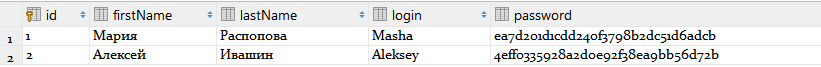
\includegraphics[scale=0.3]{img/database/before_registry_user.png} & В базе присутсвуют \\ && только два пользователя \\
	\hline 
	2 & 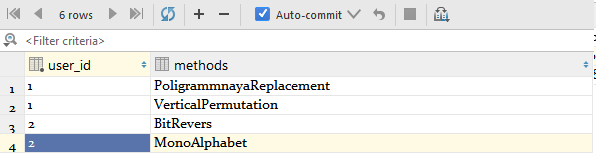
\includegraphics[scale=0.3]{img/database/before_registry_methods.png} & В базе каждому пользователю \\ && соответсвуют два метода\\
	\hline 
	3 & 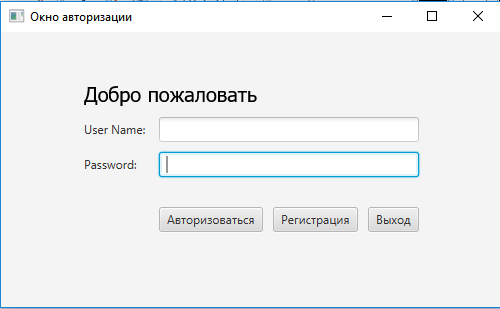
\includegraphics[scale=0.3]{img/login_form.png} & Открываем окно авторизации\\
	\hline 
	4 & 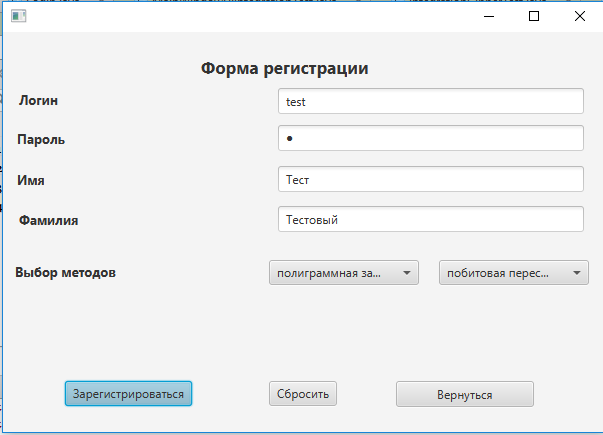
\includegraphics[scale=0.3]{img/database/before_registry_form.png} & Открываем окно регистрации \\ && и заполняем все поля\\
	\hline 
	5 & 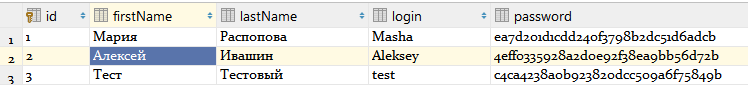
\includegraphics[scale=0.3]{img/database/after_registry_user.png} & После регистрации можно увидеть, \\ && что введенный пользователь появился в БД\\
	\hline
\end{tabular} 
\label{table:data_type1} 
\end{table}

\begin{table}[pt!]
	\caption{Тестрование регистрации пользователя}
	\centering
	\begin{tabular}{|c|c|c|}
	\hline 
	№  & Результат & Примечание \\ 
	\hline 
	6 & 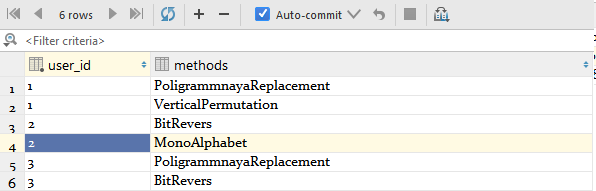
\includegraphics[scale=0.3]{img/database/after_registry_methods.png} & Так же можно увидеть, что \\ && для нового пользователя \\ && появились соответсвующие методы\\
	\hline 
	7 & 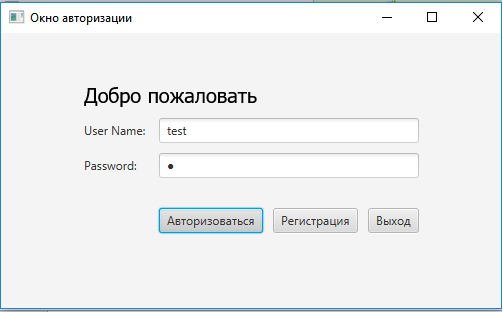
\includegraphics[scale=0.3]{img/database/authorization.png} & Открываем окно авторизации \\ && и заходим в систему под \\ && новым пользователем\\
	\hline 
	8 & 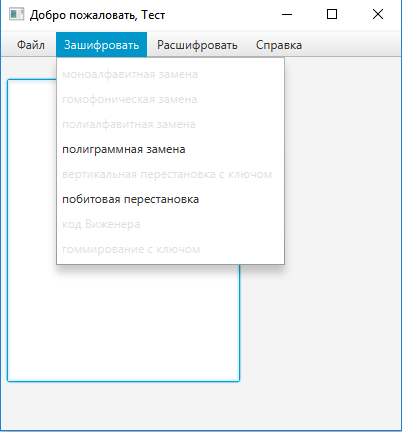
\includegraphics[scale=0.3]{img/database/main_open_methods.png} & Так же можно увидеть, \\ && что для нового пользователя появились\\ &&  соответсвующие методы шифрования\\
	\hline 
	9 & 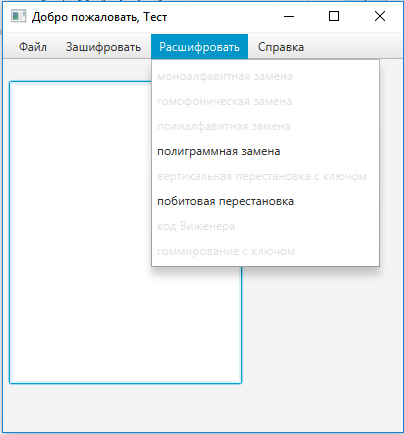
\includegraphics[scale=0.3]{img/database/main_open_methods2.png} & Так же можно увидеть, \\ && что для нового пользователя появились\\ &&  соответсвующие методы расшифрования\\
	\hline 
\end{tabular} 
\label{table:data_type2} 
\end{table}

\begin{table}[pt!]
	\caption{Тестрование сохранения в файл}
	\centering
	\begin{tabular}{|c|c|c|}
	\hline 
	№  & Результат & Примечание \\ 
	\hline 
	1 & 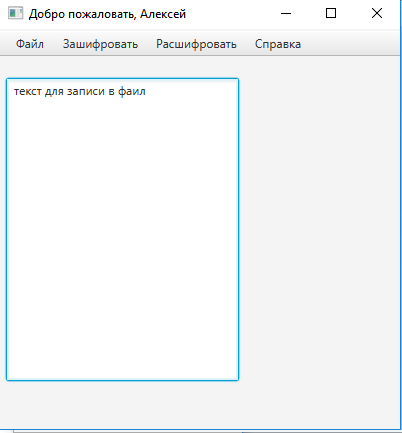
\includegraphics[scale=0.3]{img/file/open/text_open4.png} & Вводим текст в поле для \\ && ввода текста (memo) \\
	\hline 
	2 & 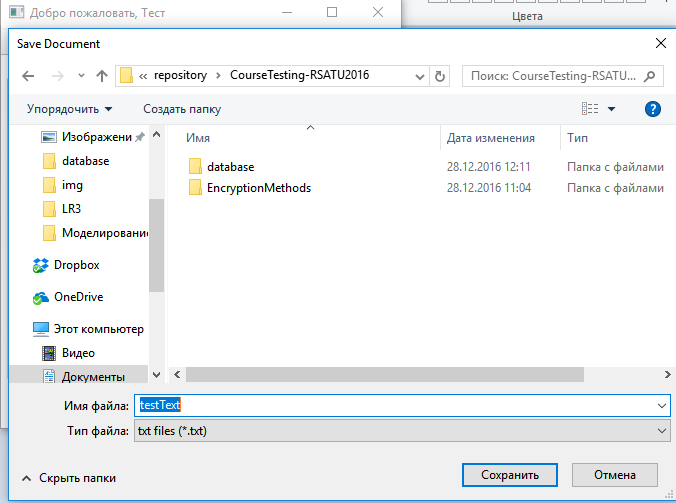
\includegraphics[scale=0.3]{img/file/save/text_path.png} & Выбираем путь, куда будет \\ && сохранен файл с текстом\\
	\hline 
	3 & 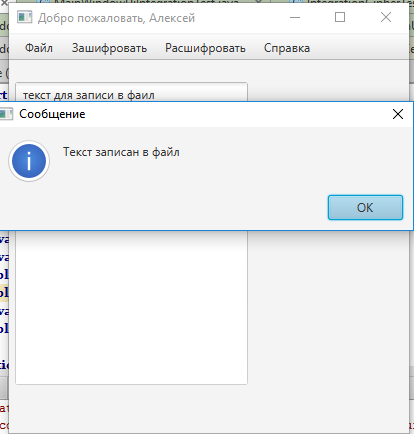
\includegraphics[scale=0.3]{img/file/save/text_okey_save.png} & Вывод сообщения о том что файл сохранен\\
	\hline 
\end{tabular} 
\label{table:data_type3} 
\end{table}

\begin{table}[pt!]
	\caption{Тестрование открытия файла}
	\centering
	\begin{tabular}{|c|c|c|}
	\hline 
	№  & Результат & Примечание \\ 
	\hline 
	1 & 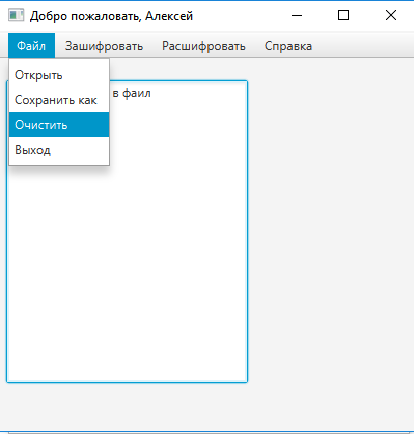
\includegraphics[scale=0.3]{img/file/open/text_clear.png} & Выбираем очистку поля ввода \\
	\hline 
	2 & 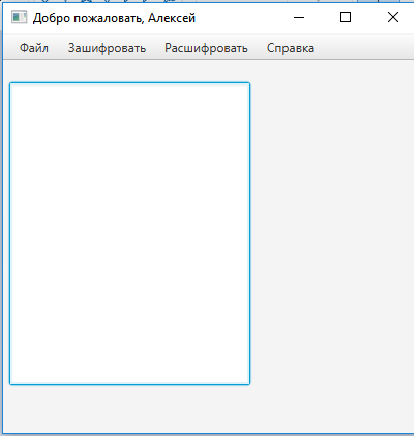
\includegraphics[scale=0.3]{img/file/open/text_clear1.png} & Видим что поле очистилось\\
	\hline 
	3 & 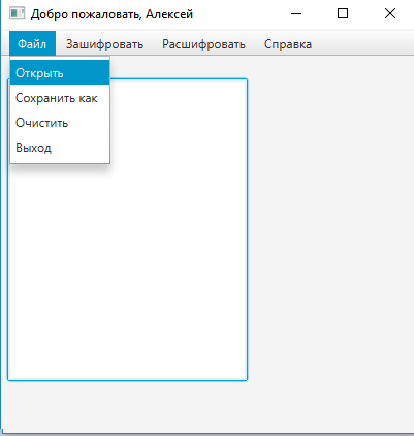
\includegraphics[scale=0.3]{img/file/open/text_open.png} & Выбираем открытие файла\\
	\hline 
\end{tabular} 
\label{table:data_type4} 
\end{table}

\begin{table}[pt!]
	\caption{Тестрование открытия файла}
	\centering
	\begin{tabular}{|c|c|c|}
	\hline 
	№  & Результат & Примечание \\ 
	\hline 
	5 & 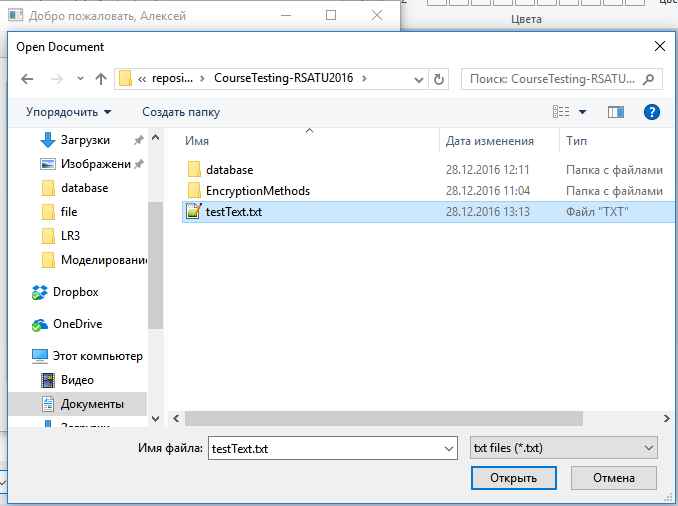
\includegraphics[scale=0.3]{img/file/open/text_open2.png} & Выбираем путь до файла\\
	\hline 
	6 & 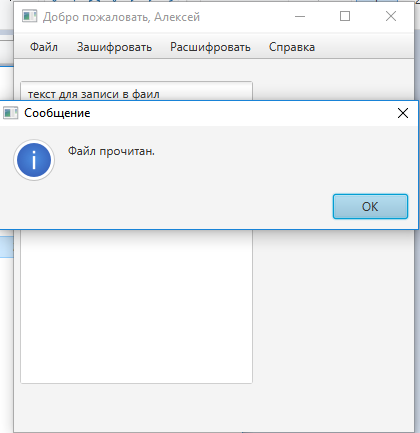
\includegraphics[scale=0.3]{img/file/open/text_open3.png} & Видим, что файл открылся\\
	\hline
	7 & 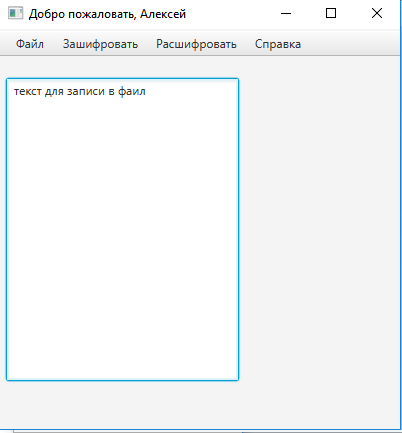
\includegraphics[scale=0.3]{img/file/open/text_open4.png} & Текст из файла в поле\\
	\hline
\end{tabular} 
\label{table:data_type5} 
\end{table}

\newpage\subsection{Результаты тестирования и выводы на данном этапе}
Результаты прохождения тестов представлены в таблицах \ref{table:system_testing_gui} - \ref{table:system_testing_by_hands}.

Все тесты были пройдены успешно, ошибок не было обнаружено.

\begin{table}[h!]
	\caption{Прохождение автоматиированных GUI тестов при системном тестировании}
	\centering
	\begin{tabular}{|c|l|l|}
	\hline 
	№ &  Название теста & Результат \\ 
	\hline 
	\multicolumn{3}{|c|}{Класс \textbf{DatabaseAndRegistryUiTest}}\\
	\hline
	1 & userExistsTest & Успешно пройден  \\
	\hline 
	\multicolumn{3}{|c|}{Класс \textbf{UserWorkingNotMethodsUiTesting}}\\
	\hline
	2 &  fullWorkTest & Успешно пройден  \\
	\hline 
	\multicolumn{3}{|c|}{Класс \textbf{UserWorkingUiTesting}}\\
	\hline
	3 & fullWorkTest & Успешно пройден  \\
	\hline
\end{tabular} 
\label{table:system_testing_gui} 
\end{table}

\begin{table}[h!]
	\caption{Прохождение ручных тестов}
	\centering
	\begin{tabular}{|c|l|l|}
	\hline 
	№ &  Название теста & Результат \\ 
	\hline
	4 & Тестирование регистрации нового пользователя & Успешно пройден  \\
	\hline
	5 &  Тестирование работы с текстовым файлом & Успешно пройден  \\
	\hline
\end{tabular} 
\label{table:system_testing_by_hands} 
\end{table}

\newpage\section*{Выводы}
\addcontentsline{toc}{section}{Выводы}
В результате выполнения курсового проекта были изучены основные принципы тестирования ПО. Так же была рассмотрена классификация по степени изолированости компонентов, при рассмотрении которой были изучены: модульное, интеграционное и системное тестирования. 
\par В ходе изучения этапов тестирования нами были разработаны классы для автоматизированного тестирования приложения, а так же было проведено комплексное ручное тестирвание приложения. В следствии, которого были установлены некоторые ошибки связаные с изначальным проектированием программы. В частности, оба алвафита при первичной разработке приложения являлись static полями класса. А когда был вынесен общий класс, для методов шифрования/расшифрования такой подход не мог является верным, т. к. каждая реализация обращалась к единым полям для всех, в следствии чего данные поля хранили в себе информацию о последнем (не том, что сейчас может использоваться) методе.
\par Так же подключение к базе данных, создавалось при первой загрузке класса, что не давало возможным подмены используемой базы на тестовую, при тестировании. Чтобы иметь возможность протестировать корректную работоспособность приложения с БД подключение было вынесено в отдельный метод, который вызывался при запуске программы. Чтобы приложение подключалось к тестовой базе данных был разработан класс - TestingDataBaseService, у которого был изменен путь к файлу БД. Экземпляр класса создавался непосредственно перед запуском окна логирования и передавался в соответсвующий метод программы, которые инициализировал требуемые поля класса для последующей работы.
\par При написании тестов была изучена и использована библиотека JUnit, а действия пользователя при работе с графическим интерфейсом моделировались с помошью библиотеки TestFX. Для этого были разработаны как автоматические, так и ручные тесты(в тех слечаях, где автоматизировать невозможно).
\par В ходе тестирования, для удобства, была переработа структура программы. Так же изначальная спецификация притерпела изменения: изначально требовалась написать программу, где информация о пользователях будет храниться в HashMap, которая константно задана в коде программы. Подобная реализая была не безопасна по следующим причина: пароли хранились в открытом виде, сама информация о пользователя хранилась в коде программы из-за чего продвинутый пользователь мог без труда получить к ней информацию. Так же для добавления нового пользователя требовалось править исходный код программы.
\par Для первоначальной спецификации были уже разработаны тесты и проведено предварительное тестирование, после всех изменений некоторые тесты стали непригодными, т. к. изначально были заточены под другую спецификацию программного продукта. Также можно сказать, что были изучены базовые принципы TDD (разработки через тестирования), т. к. изначально были написаны тесты с соответсвующей функциональности разработываемого приложения, а после изменения приложения они были запущены и не все из них были выполнены успешно, некоторые из за ошибок в коде. Например при копирования шифрования введенного пользователем пароля в формате md5 метод вызывался дважды, т. е. брался хэш от хэша, из-за чего авторизация не проходилась верно. Так же все дополнительные части приложения такие как универсальная проверка строки на пустоту, хэширования строки в формате md5, подключение к БД и создание нового пользователя, регистрация были написаны уже после написания для них соответсвующих тестов. Что помогло грамотно спроектировать программный код приложения, а так же удостоверится в корректности работы базовых функций программы.

\newpage\section*{Список литературы}
\addcontentsline{toc}{section}{Список литературы}

\begin{enumerate}
\item Канер С.  и др. Тестирование  программного  обеспечения.  Фундаментальные  концепции  
менеджмента бизнес-приложений.:  Пер.  с англ.  —  К.:  Издательство  «ДиаСофт»,  2001.  —  544  с.  
\item Бейзер Б. Тестирование черного ящика. Технологии функционального тестирования программного обеспечения и систем.  —  СПБ.: Питер, 2004.  —  318 с.: ил.
\par Интернет-источники:
\item http://www.intuit.ru/studies/courses/48/48/info
\item http://www.protesting.ru/testing/
\end{enumerate}


\newpage\section*{Приложения}
\addcontentsline{toc}{section}{Приложения}

\begin{center}
	\begin{figure}[h!]
		\centering
		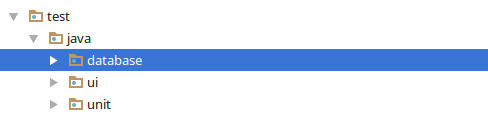
\includegraphics[scale=0.7]{img/struct1.png}
		\caption{Общая структура разработанного набора модулей}
		\label{fig:struct1}
	\end{figure}
\end{center}

\begin{center}
	\begin{figure}[h!]
		\centering
		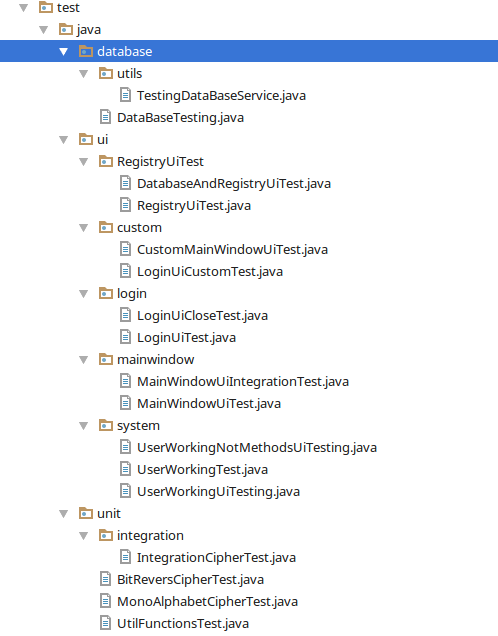
\includegraphics[scale=0.7]{img/struct2.png}
		\caption{Все модули}
		\label{fig:struct2}
	\end{figure}
\end{center}

\begin{lstlisting}[language=java, caption=код модуля TestingDataBaseService.java]
package database.utils;

import database.service.DataBaseService;
import org.hibernate.cfg.Configuration;

/**
 * Created by Алексей on 27.12.2016.
 */
public class TestingDataBaseService extends DataBaseService {
    private static String CONNECTION_TESTING_URL = "jdbc:sqlite:../database/test.db";
    private TestingDataBaseService() {
        super();
    }

    public static synchronized DataBaseService instanceDataBaseService() {
        if (service == null) {
            service = new TestingDataBaseService();
        }
        return service;
    }

    @Override
    public Configuration getSqliteConfiguration() {
        Configuration configuration = super.getSqliteConfiguration();
        configuration.setProperty("hibernate.connection.url", CONNECTION_TESTING_URL);
        return configuration;
    }

}
\end{lstlisting}

\begin{lstlisting}[language=java, caption=код модуля DataBaseTesting.java]
package database;

import database.dao.UserDao;
import database.entity.User;
import database.service.DaoFactory;
import database.service.DataBaseService;
import database.utils.TestingDataBaseService;
import org.hibernate.SessionFactory;
import org.junit.*;

import java.util.Arrays;

import static org.junit.Assert.assertEquals;
import static utils.UtilFunctions.md5Custom;

/**
 * Created by Алексей on 06.01.2017.
 */
public class DataBaseTesting {
    private static DataBaseService dataBaseService;
    private static UserDao userDao;
    private User actualUser;

    @BeforeClass
    public static void createConnectionDatabase() {
        dataBaseService = TestingDataBaseService.instanceDataBaseService();
        SessionFactory sessionFactory = dataBaseService.getSessionFactory();
        userDao = DaoFactory.getInstance(sessionFactory).getUserDao();
    }

    @AfterClass
    public static void closeConnectionDatabase() {
        dataBaseService.closeSessionFactory();
    }

    @Before
    public void createTestUser() {
        actualUser = new User().setFirstName("Тест")
                .setLastName("Тестовый")
                .setLogin("test")
                .setPassword(md5Custom("1"))
                .setMethods(Arrays.asList("BitRevers", "PoligrammnayaReplacement"));
    }

    @After
    public void deleteTestUser() {
        userDao.deleteObject(1L);
    }

    @Test
    public void createUserTest() {
        User actualUser = new User().setFirstName("Тест")
                .setLastName("Тестовый")
                .setLogin("test")
                .setPassword(md5Custom("1"))
                .setMethods(Arrays.asList("BitRevers", "PoligrammnayaReplacement"));
        userDao.addObject(actualUser);
        User expectedUser = userDao.getEntityByStringProperty("login", "test");
        assertEquals(expectedUser, actualUser);
    }


}
\end{lstlisting}

\begin{lstlisting}[language=java, caption=код модуля DatabaseAndRegistryUiTest.java]
package ui.RegistryUiTest;

import javafx.scene.control.Label;
import org.junit.Assert;
import org.junit.Test;
import ui.custom.LoginUiCustomTest;

import static org.loadui.testfx.GuiTest.find;

/**
 * Created by Алексей on 26.12.2016.
 */
public class DatabaseAndRegistryUiTest extends LoginUiCustomTest {

    @Test
    public void userExistsTest() {
        clickOn(registry);
        clickOn("#login").write("Aleksey");
        clickOn("#password").write("tesPass");
        clickOn("#signUp");
        Label outputErrorText = find("#outputErrorText");
        Assert.assertEquals(outputErrorText.getText(), "Пользователь с логином: Aleksey существует!");
        closeRegistryWindowAndTest();
    }


}
\end{lstlisting}

\begin{lstlisting}[language=java, caption=код модуля RegistryUiTest.java]
package ui.RegistryUiTest;

import javafx.fxml.FXMLLoader;
import javafx.scene.Parent;
import javafx.scene.control.Label;
import org.junit.*;
import org.loadui.testfx.GuiTest;
import org.testfx.api.FxRobot;

import java.io.IOException;

/**
 * Created by Алексей on 26.12.2016.
 */
public class RegistryUiTest extends GuiTest {
    private static FxRobot robot;
    private Label outputErrorText;

    @BeforeClass
    public static void createRobot() {
        robot = new FxRobot();
    }

    @Before
    public void getOutputErrorText() {
        outputErrorText =  find("#outputErrorText");
    }

    @After
    public void clickResetField() {
        robot.clickOn("#reset");
    }

    @Override
    protected Parent getRootNode() {
        Parent parent = null;
        try {
            parent = FXMLLoader.load(getClass().getResource("/fxml/Registry.fxml"));
            return parent;
        } catch (IOException ex) {
            // TODO ...
        }
        return parent;
    }


    @Test
    public void emptyLoginAndPasswordFieldTest() {
        robot.clickOn("#signUp").sleep(500);
        Assert.assertEquals(outputErrorText.getText(), "Не заполнены обязательные поля: Логин; Пароль; ");
    }

    @Test
    public void emptyLoginFieldTest() {
        robot.clickOn("#login").write("notEmptyLogin");
        robot.clickOn("#signUp");
        Assert.assertEquals(outputErrorText.getText(), "Не заполнены обязательные поля: Пароль; ");
    }

    @Test
    public void emptyPasswordFieldTest() {
        robot.clickOn("#password").write("tesPass");
        robot.clickOn("#signUp");
        Assert.assertEquals(outputErrorText.getText(), "Не заполнены обязательные поля: Логин; ");
    }
}
\end{lstlisting}

\begin{lstlisting}[language=java, caption=код модуля CustomMainWindowUiTest.java]
package ui.custom;

import javafx.fxml.FXMLLoader;
import javafx.scene.Parent;
import org.loadui.testfx.GuiTest;
import org.testfx.api.FxRobot;

import java.io.IOException;
import java.util.Arrays;
import java.util.List;

/**
 * Created by Алексей on 25.12.2016.
 */
public class CustomMainWindowUiTest extends GuiTest {
    protected static FxRobot robot;
    protected static List<String> methodNames;

    static {
        robot = new FxRobot();

        methodNames = Arrays.asList(
                "MonoAlphabet", "HomophonyReplacement", "PolyalphabeticReplacement",
                "PoligrammnayaReplacement", "VerticalPermutation", "BitRevers",
                "VizhinerMethod", "XOR"
        );
    }

    @Override
    protected Parent getRootNode() {
        Parent parent = null;
        try {
            parent = FXMLLoader.load(getClass().getResource("/fxml/MainWindow.fxml"));
            return parent;
        } catch (IOException ex) {
            // TODO ...
        }
        return parent;
    }
}
\end{lstlisting}

\begin{lstlisting}[language=java, caption=код модуля TestingDataBaseService.java]

\end{lstlisting}

\begin{lstlisting}[language=java, caption=код модуля LoginUiCustomTest.java]
package ui.custom;

import controller.Login;
import database.dao.UserDao;
import database.service.DaoFactory;
import database.service.DataBaseService;
import javafx.scene.control.Button;
import javafx.scene.control.PasswordField;
import javafx.scene.control.TextField;
import javafx.scene.layout.GridPane;
import javafx.scene.text.Text;
import javafx.stage.Stage;
import org.hibernate.SessionFactory;
import org.testfx.framework.junit.ApplicationTest;

import static controller.Login.GRID;
import static org.junit.Assert.assertEquals;
import static org.loadui.testfx.GuiTest.find;
import static org.loadui.testfx.GuiTest.waitUntil;
import static org.loadui.testfx.controls.impl.VisibleNodesMatcher.visible;

/**
 * Created by Алексей on 25.12.2016.
 */
public abstract class LoginUiCustomTest extends ApplicationTest {
    protected Text resultAuthorization;
    protected Button authorization;
    protected Button registry;
    protected TextField userName;
    protected PasswordField password;
    protected Stage stage;
    protected GridPane gridPane;

    protected SessionFactory sessionFactory;
    protected UserDao userDao;

    @Override
    public void start(Stage stage) throws Exception {
        this.stage = stage;
        createDatabaseConnection();
        Login.userDao = userDao;
        Login.sessionFactory = sessionFactory;
        new Login().start(stage);
        gridPane = GRID;
        resultAuthorization = find("#resultAuthorization");
        authorization = find("#authorization");
        userName = find("#login");
        password = find("#password");
        registry = find("#checkIn");
    }

    protected void createDatabaseConnection() {
        DataBaseService dataBaseService = DataBaseService.instanceDataBaseService();
        sessionFactory = dataBaseService.getSessionFactory();
        userDao = DaoFactory.getInstance(sessionFactory).getUserDao();
    }

    protected void openRegistryWindowAndTest() {
        clickOn(registry);
        assertEquals(gridPane.isDisable(), true);
        waitUntil("#registryPane", visible());
    }

    protected void closeRegistryWindowAndTest() {
        clickOn("#back");
        assertEquals(gridPane.isDisable(), false);
    }
}
\end{lstlisting}

\begin{lstlisting}[language=java, caption=код модуля LoginUiCloseTest.java]
package ui.login;

import javafx.scene.paint.Color;
import org.junit.Test;
import ui.custom.LoginUiCustomTest;

import static controller.Login.sessionFactory;
import static org.junit.Assert.assertEquals;
import static org.testfx.api.FxAssert.verifyThat;
import static org.testfx.matcher.base.NodeMatchers.hasText;

/**
 * Created by Алексей on 25.12.2016.
 */
public class LoginUiCloseTest extends LoginUiCustomTest {
    @Test
    public void threeWrongAuthorizationTest() {
        for (int i = 0; i < 3; i++) {
            clickOn(userName).write("Aleksey");
            clickOn(password).write("tttt");
            clickOn(authorization).sleep(100);
            verifyThat(resultAuthorization, hasText("Не верный пароль"));
            assertEquals(resultAuthorization.getFill(), Color.FIREBRICK);
            userName.clear();
            password.clear();
        }
        assertEquals(stage.isShowing(), false);
        assertEquals(sessionFactory.isClosed(), true);
    }
}
\end{lstlisting}

\begin{lstlisting}[language=java, caption=код модуля LoginUiTest.java]
package ui.login;

import javafx.scene.paint.Color;
import org.junit.Before;
import org.junit.Test;
import ui.custom.LoginUiCustomTest;

import static controller.Login.sessionFactory;
import static org.junit.Assert.assertEquals;
import static org.loadui.testfx.GuiTest.waitUntil;
import static org.loadui.testfx.controls.impl.VisibleNodesMatcher.visible;
import static org.testfx.api.FxAssert.verifyThat;
import static org.testfx.matcher.base.NodeMatchers.hasText;

/**
 * Created by Алексей on 20.12.2016.
 */
public class LoginUiTest extends LoginUiCustomTest {

    @Before
    public void checkOpenSession() {
        assertEquals(sessionFactory.isClosed(), false);
    }

    @Test
    public void openMainWindowTest() {
        assertEquals(sessionFactory.isClosed(), false);
        clickOn(userName).write("Aleksey");
        clickOn(password).write("yui");
        clickOn(authorization);
        verifyThat(resultAuthorization, hasText("Пароль верный"));
        assertEquals(resultAuthorization.getFill(), Color.GREEN);
        waitUntil("#AnchorPane", visible());
    }

    @Test
    public void wrongAuthorizationTest() {
        assertEquals(sessionFactory.isClosed(), false);
        clickOn(userName).write("Aleksey");
        clickOn(password).write("retdfgdfh");
        clickOn(authorization);
        verifyThat(resultAuthorization, hasText("Не верный пароль"));
        assertEquals(resultAuthorization.getFill(), Color.FIREBRICK);
    }

    @Test
    public void openRegistryWindowTest() {
        openRegistryWindowAndTest();
        closeRegistryWindowAndTest();
    }

    @Test
    public void thisUserDoesntExistTest() {
        assertEquals(sessionFactory.isClosed(), false);
        clickOn(userName).write("ТестНик");
        clickOn(password).write("tttt");
        clickOn(authorization);
        verifyThat(resultAuthorization, hasText("Такого пользователя не существует"));
        assertEquals(resultAuthorization.getFill(), Color.FIREBRICK);
    }
}
\end{lstlisting}

\begin{lstlisting}[language=java, caption=код модуля MainWindowUiIntegrationTest.java]
package ui.mainwindow;

import controller.MainWindowController;
import javafx.scene.control.TextArea;
import org.junit.*;
import ui.custom.CustomMainWindowUiTest;

import java.util.Arrays;

/**
 * Created by Алексей on 25.12.2016.
 */
public class MainWindowUiIntegrationTest extends CustomMainWindowUiTest {
    private TextArea textArea;
    String actualText;

    @BeforeClass
    public static void mainWindowSettings() {
        MainWindowController.nameMethods = Arrays.asList(
                methodNames.get(0), methodNames.get(5)
        );
    }

    @Before
    public void findTextArea() {
        textArea = find("#textArea");
        actualText = "специальныи текст для тестов";
        robot.clickOn(textArea).write(actualText);
    }

    @After
    public void clearTextArea() {
        textArea.clear();
    }

    @Test
    public void integrationCipherEqualsTest() {
        robot.clickOn("#encodeMenu").clickOn("#encodeMonoAlphabet")
                .clickOn("#txtFieldDialog").write('4').clickOn("#okDialog");
        robot.clickOn("#decodeMenu").clickOn("#decodeBitRevers")
                .clickOn("#txtFieldDialog").write("32451").clickOn("#okDialog");
        robot.clickOn("#encodeMenu").clickOn("#encodeBitRevers")
                .clickOn("#txtFieldDialog").write("32451").clickOn("#okDialog");
        robot.clickOn("#decodeMenu").clickOn("#decodeMonoAlphabet")
                .clickOn("#txtFieldDialog").write('4').clickOn("#okDialog");
        Assert.assertEquals(textArea.getText(), actualText);
    }

    @Test
    public void integrationCipherNotEqualsTest() {
        robot.clickOn("#encodeMenu").clickOn("#encodeMonoAlphabet")
                .clickOn("#txtFieldDialog").write('4').clickOn("#okDialog");
        robot.clickOn("#decodeMenu").clickOn("#decodeBitRevers")
                .clickOn("#txtFieldDialog").write("32451").clickOn("#okDialog");
        String testText = textArea.getText();
        robot.clickOn("#decodeMenu").clickOn("#decodeBitRevers")
                .clickOn("#txtFieldDialog").write("52341").clickOn("#okDialog");
        Assert.assertNotEquals(textArea.getText(), testText);
    }

    @Test
    public void  integrationDeepCipherEqualsTest() {
        robot.clickOn("#encodeMenu").clickOn("#encodeMonoAlphabet")
                .clickOn("#txtFieldDialog").write("2").clickOn("#okDialog");
        robot.clickOn("#encodeMenu").clickOn("#encodeBitRevers")
                .clickOn("#txtFieldDialog").write("53241").clickOn("#okDialog");
        Assert.assertNotEquals(textArea.getText(), actualText);
        robot.clickOn("#decodeMenu").clickOn("#decodeMonoAlphabet")
                .clickOn("#txtFieldDialog").write('3').clickOn("#okDialog");
        robot.clickOn("#decodeMenu").clickOn("#decodeBitRevers")
                .clickOn("#txtFieldDialog").write("24531").clickOn("#okDialog");
        Assert.assertNotEquals(textArea.getText(), actualText);
        robot.clickOn("#encodeMenu").clickOn("#encodeBitRevers")
                .clickOn("#txtFieldDialog").write("24531").clickOn("#okDialog");
        robot.clickOn("#encodeMenu").clickOn("#encodeMonoAlphabet")
                .clickOn("#txtFieldDialog").write('3').clickOn("#okDialog");
        Assert.assertNotEquals(textArea.getText(), actualText);
        robot.clickOn("#decodeMenu").clickOn("#decodeBitRevers")
                .clickOn("#txtFieldDialog").write("53241").clickOn("#okDialog");
        robot.clickOn("#decodeMenu").clickOn("#decodeMonoAlphabet")
                .clickOn("#txtFieldDialog").write('2').clickOn("#okDialog");
        Assert.assertEquals(textArea.getText(), actualText);
    }
}
\end{lstlisting}

\begin{lstlisting}[language=java, caption=код модуля MainWindowUiTest.java]
package ui.mainwindow;

import javafx.fxml.FXMLLoader;
import javafx.scene.Parent;
import javafx.scene.control.TextArea;
import org.junit.Before;
import org.junit.Test;
import ui.custom.CustomMainWindowUiTest;

import java.io.IOException;

import static org.testfx.api.FxAssert.verifyThat;
import static org.testfx.matcher.base.NodeMatchers.hasText;

/**
 * Created by Алексей on 22.12.2016.
 */
public class MainWindowUiTest extends CustomMainWindowUiTest {
    private TextArea textArea;

    @Before
    public void findTextArea() {
        textArea = find("#textArea");
    }

    @Override
    protected Parent getRootNode() {
        Parent parent = null;
        try {
            parent = FXMLLoader.load(getClass().getResource("/fxml/MainWindow.fxml"));
            return parent;
        } catch (IOException ex) {
            // TODO ...
        }
        return parent;
    }

    @Test
    public void writeInTextAreaTest() {
        robot.clickOn(textArea).write("авыаыва");
        verifyThat(textArea, hasText("авыаыва"));
    }

    @Test
    public void clickAllEncodeMenuTest() {
        robot.clickOn("#encodeMenu");
        clickAllMethodsMenu("encode");
        robot.clickOn("#encodeMenu");
    }

    @Test
    public void clickAllDecodeMenuTest() {
        robot.clickOn("#decodeMenu");
        clickAllMethodsMenu("decode");
        robot.clickOn("#decodeMenu");
    }

    private static void clickAllMethodsMenu(String variantName) {
        String itemId;
        for (String name : methodNames) {
            itemId = "#" + variantName + name;
            robot.clickOn(itemId);
        }
    }
    @Test
    public void clearTextArea() {
        String testText = "текстовый текст, для проверки очистки области ввода текста";
        robot.clickOn(textArea).write(testText);
        verifyThat(textArea, hasText(testText));
        robot.clickOn("#fileMenu").clickOn("#clear");
        verifyThat(textArea, hasText(""));
    }
}
\end{lstlisting}

\begin{lstlisting}[language=java, caption=код модуля UserWorkingNotMethodsUiTesting.java]
package ui.system;

import controller.MainWindowController;
import org.junit.Test;

import static org.junit.Assert.assertEquals;
import static org.testfx.api.FxAssert.verifyThat;
import static org.testfx.matcher.base.NodeMatchers.hasText;

/**
 * Created by Алексей on 06.01.2017.
 */
public class UserWorkingNotMethodsUiTesting extends UserWorkingTest {

    @Test
    public void fullWorkTest() {
        openRegistryWindowAndTest();
        registryTestUser();
        authorizationTestUser();
        assertEquals(MainWindowController.stage.getTitle(), "Добро пожаловать, Тест");
        writeTextArea();
        clickMethodTest("#encodeHomophonyReplacement");
        checkDialogAndClose();
        clickMethodTest("#encodeVizhinerMethod");
        checkDialogAndClose();
    }

    private void registryTestUser() {
        clickOn("#login").write("testUser2");
        clickOn("#password").write("1");
        clickOn("#firstName").write("Тест");
        clickOn("#lastName").write("Тестовый");
        clickOn("#firstMethod").clickOn("гомофоническая замена");
        clickOn("#secondMethod").clickOn("код Виженера");
        clickOn("#signUp");
    }

    private void authorizationTestUser() {
        clickOn(userName).write("testUser2");
        clickOn(password).write("1");
        openMainWindowTest();
    }

    private void clickMethodTest(String methodName) {
        clickOn("#encodeMenu").clickOn(methodName);
    }

    private void checkDialogAndClose() {
        verifyThat("#labelDialog", hasText("Метод не реализован"));
        clickOn("#okDialog");
    }
}
\end{lstlisting}

\begin{lstlisting}[language=java, caption=код модуля UserWorkingTest.java]
package ui.system;

import database.service.DaoFactory;
import database.service.DataBaseService;
import database.utils.TestingDataBaseService;
import javafx.scene.paint.Color;
import org.junit.After;
import ui.custom.LoginUiCustomTest;

import static org.junit.Assert.assertEquals;
import static org.loadui.testfx.GuiTest.waitUntil;
import static org.loadui.testfx.controls.impl.VisibleNodesMatcher.visible;
import static org.testfx.api.FxAssert.verifyThat;
import static org.testfx.matcher.base.NodeMatchers.hasText;

/**
 * Created by Алексей on 06.01.2017.
 */
public class UserWorkingTest extends LoginUiCustomTest {
    protected String actualText = "специальныи текст для тестов";

    @After
    public void deleteTestUser() {
        userDao.deleteObject(1L);
    }

    @Override
    protected void createDatabaseConnection() {
        DataBaseService dataBaseService = TestingDataBaseService.instanceDataBaseService();
        sessionFactory = dataBaseService.getSessionFactory();
        userDao = DaoFactory.getInstance(sessionFactory).getUserDao();
    }

    protected void writeTextArea() {
        clickOn("#textArea").write(actualText);
    }

    protected void openMainWindowTest() {
        clickOn(authorization);
        verifyThat(resultAuthorization, hasText("Пароль верный"));
        assertEquals(resultAuthorization.getFill(), Color.GREEN);
        waitUntil("#AnchorPane", visible());
    }

}
\end{lstlisting}

\begin{lstlisting}[language=java, caption=код модуля UserWorkingUiTesting.java]
package ui.system;

import controller.MainWindowController;
import javafx.scene.control.TextArea;
import org.junit.Assert;
import org.junit.Test;

import static org.junit.Assert.assertEquals;
import static org.loadui.testfx.GuiTest.find;

/**
 * Created by Алексей on 06.01.2017.
 */
public class UserWorkingUiTesting extends UserWorkingTest {
    @Test
    public void fullWorkTest() {
        openRegistryWindowAndTest();
        registryTestUser();
        authorizationTestUser();
        assertEquals(MainWindowController.stage.getTitle(), "Добро пожаловать, Неизвестный");
        writeTextArea();
        integrationCipherEqualsTest();
    }

    private void registryTestUser() {
        clickOn("#login").write("testUser");
        clickOn("#password").write("1");
        clickOn("#firstMethod").clickOn("побитовая перестановка");
        clickOn("#signUp");
    }

    private void authorizationTestUser() {
        clickOn(userName).write("testUser");
        clickOn(password).write("1");
        openMainWindowTest();
    }

    private void integrationCipherEqualsTest() {
        clickOn("#encodeMenu").clickOn("#encodeMonoAlphabet")
                .clickOn("#txtFieldDialog").write("24").clickOn("#okDialog");
        clickOn("#decodeMenu").clickOn("#decodeBitRevers")
                .clickOn("#txtFieldDialog").write("42351").clickOn("#okDialog");
        clickOn("#encodeMenu").clickOn("#encodeBitRevers")
                .clickOn("#txtFieldDialog").write("42351").clickOn("#okDialog");
        clickOn("#decodeMenu").clickOn("#decodeMonoAlphabet")
                .clickOn("#txtFieldDialog").write("24").clickOn("#okDialog");
        TextArea textArea = find("#textArea");
        Assert.assertEquals(textArea.getText(), actualText);
    }
}
\end{lstlisting}

\begin{lstlisting}[language=java, caption=код модуля IntegrationCipherTest.java]
package unit.integration;

import encryptionMethods.base.SubstitutionCipher;
import encryptionMethods.bitrevers.BitReversCipher;
import encryptionMethods.monoAlphabet.MonoAlphabetCipher;
import org.junit.Assert;
import org.junit.Before;
import org.junit.BeforeClass;
import org.junit.Test;

/**
 * Created by Алексей on 22.12.2016.
 */
public class IntegrationCipherTest {
    private static SubstitutionCipher<Integer> monoAlphabet;
    private static SubstitutionCipher<String> bitRevers;
    private String actualText;

    @BeforeClass
    public static void test() {
        monoAlphabet = new MonoAlphabetCipher();
        bitRevers = new BitReversCipher();
    }

    @Before
    public void createCipherClass() {
        actualText = "специальныи текст для тестов";
    }

    @Test
    public void integrationCipherEqualsTest() {
        monoAlphabet.calculationPrivateAlphabet(4);
        bitRevers.calculationPrivateAlphabet("32451");
        String expectedText = monoAlphabet.encodeText(actualText);
        expectedText = bitRevers.decodeText(expectedText);
        expectedText = bitRevers.encodeText(expectedText);
        expectedText = monoAlphabet.decodeText(expectedText);
        Assert.assertEquals(expectedText, actualText);
    }

    @Test
    public void  integrationCipherNotEqualsTest() {
        monoAlphabet.calculationPrivateAlphabet(4);
        bitRevers.calculationPrivateAlphabet("32451");
        String testText = monoAlphabet.encodeText(actualText);
        testText = bitRevers.decodeText(testText);
        bitRevers.calculationPrivateAlphabet("52341");
        String expectedText = bitRevers.encodeText(testText);
        Assert.assertNotEquals(expectedText, testText);
    }

    @Test
    public void  integrationDeepCipherEqualsTest() {
        monoAlphabet.calculationPrivateAlphabet(2);
        String expectedText = monoAlphabet.encodeText(actualText);

        bitRevers.calculationPrivateAlphabet("53241");
        expectedText = bitRevers.encodeText(expectedText);
        Assert.assertNotEquals(expectedText, actualText);

        monoAlphabet.calculationPrivateAlphabet(3);
        expectedText = monoAlphabet.decodeText(expectedText);

        bitRevers.calculationPrivateAlphabet("24531");
        expectedText = bitRevers.decodeText(expectedText);
        Assert.assertNotEquals(expectedText, actualText);

        expectedText = bitRevers.encodeText(expectedText);
        expectedText = monoAlphabet.encodeText(expectedText);
        Assert.assertNotEquals(expectedText, actualText);

        bitRevers.calculationPrivateAlphabet("53241");
        expectedText = bitRevers.decodeText(expectedText);

        monoAlphabet.calculationPrivateAlphabet(2);
        expectedText = monoAlphabet.decodeText(expectedText);

        Assert.assertEquals(expectedText, actualText);
    }
}
\end{lstlisting}

\begin{lstlisting}[language=java, caption=код модуля BitReversCipherTest.java]
package unit;

import encryptionMethods.base.SubstitutionCipher;
import encryptionMethods.bitrevers.BitReversCipher;
import org.junit.After;
import org.junit.Assert;
import org.junit.Before;
import org.junit.Test;

import static org.junit.Assert.assertArrayEquals;
import static org.junit.Assert.assertEquals;

/**
 * Created by Алексей on 19.12.2016.
 */
public class BitReversCipherTest {
    private SubstitutionCipher bitReversCipher;

    @Before
    public void beforeTest() {
        bitReversCipher = new BitReversCipher();
    }

    @After
    public void afterTest() {
        bitReversCipher = null;
    }

    @Test
    public void testCalculationPrivateAlphabetEqualsOpenAlphabet() {
        char[] actuals = {' ', 'а', 'б', 'в', 'г', 'д', 'е', 'ж', 'з', 'и', 'к', 'л', 'м', 'н', 'о', 'п', 'р', 'с', 'т', 'у', 'ф', 'х', 'ц', 'ч', 'ш', 'щ', 'ъ', 'ы', 'ь', 'э', 'ю', 'я'};
        bitReversCipher.calculationPrivateAlphabet("12345");
        assertArrayEquals(bitReversCipher.getPrivateAlphabet(), actuals);
        assertArrayEquals(bitReversCipher.getOpenAlphabet(), actuals);
        assertArrayEquals(bitReversCipher.getOpenAlphabet(), bitReversCipher.getOpenAlphabet());
    }

    @Test
    public void testCalculationPrivateAlphabet() {
        char[] actuals = {' ', 'р', 'з', 'ш', 'г', 'ф', 'м', 'ь', 'б', 'т', 'к', 'ъ', 'е', 'ц', 'о', 'ю', 'а', 'с', 'и', 'щ', 'д', 'х', 'н', 'э', 'в', 'у', 'л', 'ы', 'ж', 'ч', 'п', 'я'};
        bitReversCipher.calculationPrivateAlphabet("54321");
        assertArrayEquals(bitReversCipher.getPrivateAlphabet(), actuals);
    }

    @Test
    public void testFirstElementPrivateAlphabetAtAnyKey() {
        bitReversCipher.calculationPrivateAlphabet("54321");
        assertEquals(bitReversCipher.getPrivateAlphabet()[0], ' ');
        bitReversCipher.calculationPrivateAlphabet("53241");
        assertEquals(bitReversCipher.getPrivateAlphabet()[0], ' ');
        bitReversCipher.calculationPrivateAlphabet("13425");
        assertEquals(bitReversCipher.getPrivateAlphabet()[0], ' ');
        bitReversCipher.calculationPrivateAlphabet("31245");
        assertEquals(bitReversCipher.getPrivateAlphabet()[0], ' ');
    }

    @Test
    public void testLastElementPrivateAlphabetAtAnyKey() {
        bitReversCipher.calculationPrivateAlphabet("54321");
        assertEquals(bitReversCipher.getPrivateAlphabet()[31], 'я');
        bitReversCipher.calculationPrivateAlphabet("53241");
        assertEquals(bitReversCipher.getPrivateAlphabet()[31], 'я');
        bitReversCipher.calculationPrivateAlphabet("13425");
        assertEquals(bitReversCipher.getPrivateAlphabet()[31], 'я');
        bitReversCipher.calculationPrivateAlphabet("31245");
        assertEquals(bitReversCipher.getPrivateAlphabet()[31], 'я');
    }

    @Test
    public void testEncode() {
        bitReversCipher.calculationPrivateAlphabet("54321");
        assertEquals(bitReversCipher.encodeText("тест"), "имси");
    }

    @Test
    public void testEncodeDecode() {
        bitReversCipher.calculationPrivateAlphabet("54321");
        String encode = bitReversCipher.encodeText("тест");
        assertEquals(bitReversCipher.decodeText(encode), "тест");
    }

    @Test(expected = IndexOutOfBoundsException.class)
    public void testWrongValueForCalculationPrivateAlphabet() {
        bitReversCipher.calculationPrivateAlphabet("00000");
    }

    @Test(expected = ClassCastException.class)
    public void testWrongArgumentForCalculationPrivateAlphabet() {
        bitReversCipher.calculationPrivateAlphabet(1213234);
    }

    @Test
    public void testWrongCharInEncodeAndDecodeText() {
        bitReversCipher.calculationPrivateAlphabet("54321");
        Assert.assertEquals(bitReversCipher.encodeText("tttt"), "Недопустимый символ. Шифрование не возможно");
        Assert.assertEquals(bitReversCipher.encodeText("й"), "Недопустимый символ. Шифрование не возможно");
        Assert.assertEquals(bitReversCipher.encodeText("ё"), "Недопустимый символ. Шифрование не возможно");
        Assert.assertEquals(bitReversCipher.encodeText("-"), "Недопустимый символ. Шифрование не возможно");
        Assert.assertEquals(bitReversCipher.encodeText("+"), "Недопустимый символ. Шифрование не возможно");
        Assert.assertEquals(bitReversCipher.decodeText("tttt"), "Недопустимый символ. Расшифровка не возможно");
        Assert.assertEquals(bitReversCipher.decodeText("й"), "Недопустимый символ. Расшифровка не возможно");
        Assert.assertEquals(bitReversCipher.decodeText("ё"), "Недопустимый символ. Расшифровка не возможно");
        Assert.assertEquals(bitReversCipher.decodeText("-"), "Недопустимый символ. Расшифровка не возможно");
        Assert.assertEquals(bitReversCipher.decodeText("+"), "Недопустимый символ. Расшифровка не возможно");
    }
}
\end{lstlisting}

\begin{lstlisting}[language=java, caption=код модуля MonoAlphabetCipherTest.java]
package unit;

import encryptionMethods.base.SubstitutionCipher;
import encryptionMethods.monoAlphabet.MonoAlphabetCipher;
import org.junit.After;
import org.junit.Assert;
import org.junit.Before;
import org.junit.Test;

import static org.junit.Assert.assertArrayEquals;
import static org.junit.Assert.assertEquals;

/**
 * Created by Алексей on 19.12.2016.
 */
public class MonoAlphabetCipherTest {
    private SubstitutionCipher monoAlphabetCipher;

    @Before
    public void beforeTest() {
        monoAlphabetCipher = new MonoAlphabetCipher();
    }

    @After
    public void afterTest() {
        monoAlphabetCipher = null;
    }

    @Test(expected = NullPointerException.class)
    public void testNullCalculationPrivateAlphabet() {
        monoAlphabetCipher.calculationPrivateAlphabet(null);
    }

    @Test(expected = ClassCastException.class)
    public void testWrongArgumentCalculationPrivateAlphabet() {
        monoAlphabetCipher.calculationPrivateAlphabet("test");
    }

    @Test
    public void testCalculationPrivateAlphabet() {
        char[] actuals = {' ', 'а', 'б', 'в', 'г', 'д', 'е', 'ж', 'з', 'и', 'к', 'л', 'м', 'н', 'о', 'п', 'р', 'с', 'т', 'у', 'ф', 'х', 'ц', 'ч', 'ш', 'щ', 'ъ', 'ы', 'ь', 'э', 'ю', 'я'};
        monoAlphabetCipher.calculationPrivateAlphabet(0);
        assertArrayEquals(monoAlphabetCipher.getPrivateAlphabet(), actuals);
        assertArrayEquals(monoAlphabetCipher.getOpenAlphabet(), actuals);
        assertArrayEquals(monoAlphabetCipher.getOpenAlphabet(), monoAlphabetCipher.getOpenAlphabet());
    }

    @Test
    public void testCalculationPrivateAlphabetCaesarCipher() {
        char[] actuals = {'в', 'г', 'д', 'е', 'ж', 'з', 'и', 'к', 'л', 'м', 'н', 'о', 'п', 'р', 'с', 'т', 'у', 'ф', 'х', 'ц', 'ч', 'ш', 'щ', 'ъ', 'ы', 'ь', 'э', 'ю', 'я', ' ', 'а', 'б'};
        monoAlphabetCipher.calculationPrivateAlphabet(3);
        assertArrayEquals(monoAlphabetCipher.getPrivateAlphabet(), actuals);
    }

    @Test
    public void testEncodeText() {
        monoAlphabetCipher.calculationPrivateAlphabet(3);
        assertEquals(monoAlphabetCipher.encodeText("тест"), "хифх");
    }

    @Test
    public void testEncodeAndDecode() {
        monoAlphabetCipher.calculationPrivateAlphabet(30);
        String encode = monoAlphabetCipher.encodeText("тест");
        assertEquals("тест", monoAlphabetCipher.decodeText(encode));
    }

    @Test
    public void testWrongCharInEncodeAndDecodeText() {
        monoAlphabetCipher.calculationPrivateAlphabet(1);
        Assert.assertEquals(monoAlphabetCipher.encodeText("tttt"), "Недопустимый символ. Шифрование не возможно");
        Assert.assertEquals(monoAlphabetCipher.encodeText("й"), "Недопустимый символ. Шифрование не возможно");
        Assert.assertEquals(monoAlphabetCipher.encodeText("ё"), "Недопустимый символ. Шифрование не возможно");
        Assert.assertEquals(monoAlphabetCipher.encodeText("-"), "Недопустимый символ. Шифрование не возможно");
        Assert.assertEquals(monoAlphabetCipher.encodeText("+"), "Недопустимый символ. Шифрование не возможно");
        Assert.assertEquals(monoAlphabetCipher.decodeText("tttt"), "Недопустимый символ. Расшифровка не возможно");
        Assert.assertEquals(monoAlphabetCipher.decodeText("й"), "Недопустимый символ. Расшифровка не возможно");
        Assert.assertEquals(monoAlphabetCipher.decodeText("ё"), "Недопустимый символ. Расшифровка не возможно");
        Assert.assertEquals(monoAlphabetCipher.decodeText("-"), "Недопустимый символ. Расшифровка не возможно");
        Assert.assertEquals(monoAlphabetCipher.decodeText("+"), "Недопустимый символ. Расшифровка не возможно");
    }
}
\end{lstlisting}

\begin{lstlisting}[language=java, caption=код модуля UtilFunctionsTest.java]
package unit;

import org.junit.Test;

import static org.junit.Assert.assertEquals;
import static utils.UtilFunctions.isNullString;
import static utils.UtilFunctions.md5Custom;

/**
 * Created by Алексей on 25.12.2016.
 */
public class UtilFunctionsTest {

    @Test
    public void md5EqualsTesting() {
        String expected = md5Custom("1");
        assertEquals(expected, "c4ca4238a0b923820dcc509a6f75849b");
        expected = md5Custom("md5test");
        assertEquals(expected, "82da61aa724b5d149a9c5dc8682c2a45");
        expected = md5Custom("абра-кадбра, магия какая-то");
        assertEquals(expected, "783e47ca544ddf34ccce81b524adbbe3");
    }

    @Test
    public void md5NullArgument() {
        assertEquals(md5Custom(null), "");
    }

    @Test
    public void isNullStringTest() {
        assertEquals(isNullString(null), true);
        assertEquals(isNullString(""), true);
        assertEquals(isNullString("          "), true);
        assertEquals(isNullString("    dsfsdf   "), false);
        assertEquals(isNullString("тестовое значение"), false);
        assertEquals(isNullString(" "), true);
    }
}
\end{lstlisting}


\end{document}